% -*- mode: latex; mode: reftex; mode: auto-fill; mode: flyspell; coding: utf-8; tex-command: "pdflatex.sh" -*-

\documentclass[oneside,11pt]{memoir}

% -*- mode: latex; mode: reftex; mode: auto-fill; mode: flyspell; coding: utf-8; -*-

%%%%%%%%%%%%%%%%%%%%%%%%%%%%%%%%%%%%%%%%%%%%%%%%%%%%%%%%%%%%%%%%%%%%%%%%%%%%%%%%%%%%%%%%%%%
\usepackage{ctex}
\usepackage{amsmath}
\usepackage{amssymb}
\usepackage{dsfont}
\usepackage{ifthen}
\usepackage{caption}

\let\ordinal\relax
\usepackage[us]{datetime}
\newdateformat{dotdate}{\THEYEAR.\twodigit{\THEMONTH}.\twodigit{\THEDAY}}

\usepackage{imakeidx}
\makeindex[columns=1]

\usepackage{enumitem}
\setlist[itemize]{leftmargin=0pt,itemindent=1em,itemsep=2ex}
\setlist{nosep} % or \setlist{noitemsep} to leave space around whole list

\usepackage[utf8]{inputenc}
\usepackage[T1]{fontenc}
\usepackage[osf]{libertine}
\usepackage{microtype}

\usepackage[
  linktocpage=true,
  unicode=true,
  bookmarks=true,
  bookmarksnumbered=false,
  bookmarksopen=false,
  breaklinks=true,
  pdfborder={0 0 1},
  backref=page,
  colorlinks=true,
  linkcolor=links,
  urlcolor=links,
  citecolor=links,
  hypertexnames=false, % to avoid errors with autonum
]{hyperref} % PDF meta-information specification

\urlstyle{same}

\usepackage[object=vectorian]{pgfornament}
\def\textsep{%
\vskip1.5ex

\centerline{\pgfornament[anchor=center,ydelta=0pt,width=2cm]{82}}

\vskip0.5ex
}

\AddToHook{cmd/section/before}{\clearpage}
\usepackage[section]{placeins}

\usepackage{xspace}
\def\wordfig{Figure\xspace}
\def\wordeq{Equation\xspace}
\def\wordtable{Table\xspace}
\def\wordchap{Chapter\xspace}

\let\oldcenter\center
\let\oldendcenter\endcenter
\renewenvironment{center}{\setlength\topsep{0pt}\oldcenter}{\oldendcenter}

\usepackage{environ}
\NewEnviron{hardcenter}{\makebox[\textwidth][c]{\BODY}}

%%%%%%%%%%%%%%%%%%%%%%%%%%%%%%%%%%%%%%%%%%%%%%%%%%%%%%%%%%%%%%%%%%%%%%%%%%%%%%%%%%%%%%%%%%%
% Math
%%%%%%%%%%%%%%%%%%%%%%%%%%%%%%%%%%%%%%%%%%%%%%%%%%%%%%%%%%%%%%%%%%%%%%%%%%%%%%%%%%%%%%%%%%%

\usepackage{amsmath}
\usepackage{amssymb}
\usepackage{dsfont}
\usepackage{mleftright}

\setlength{\thinmuskip}{1.5mu} % by default it is equal to 3 mu
\setlength{\medmuskip}{2mu} % by default it is equal to 4 mu
\setlength{\thickmuskip}{3.5mu} % by default it is equal to 5 mu

\makeatletter
\DeclareFontEncoding{LS1}{}{}
\DeclareFontSubstitution{LS1}{stix}{m}{n}
\DeclareMathAlphabet{\mathcal}{LS1}{stixscr}{m}{n}
\makeatother

%%%%%%%%%%%%%%%%%%%%%%%%%%%%%%%%%%%%%%%%%%%%%%%%%%%%%%%%%%%%%%%%%%%%%%

\newcommand{\inputgenerated}[1]{%
  \IfFileExists{#1}{\input{#1}}{%
    \errmessage{Cannot find "#1", compile with -shell-escape}\stop}%
}

%\newcommand{\gradient}[2]{{\nabla\!}_{#1 \mid #2}}
\newcommand{\gradient}[2]{{\nabla\!#1}_{\mid #2}}

\def\given{\,\middle\vert\,}
\newcommand{\proba}{{P}}
\newcommand{\seq}{{S}}
\newcommand{\expect}{\mathds{E}}
\newcommand{\variance}{\mathds{V}}
\newcommand{\empexpect}{\hat{\mathds{E}}}
\newcommand{\mutinf}{\mathds{I}}
\newcommand{\empmutinf}{\hat{\mathds{I}}}
\newcommand{\entropy}{\mathds{H}}
\newcommand{\empentropy}{\hat{\mathds{H}}}
\newcommand{\ganG}{\mathbf{G}}
\newcommand{\ganD}{\mathbf{D}}
\newcommand{\ganF}{\mathbf{F}}

\newcommand{\dkl}{\mathds{D}_{\mathsf{KL}}}
\newcommand{\djs}{\mathds{D}_{\mathsf{JS}}}

\newcommand*{\vertbar}{\rule[-1ex]{0.5pt}{2.5ex}}
\newcommand*{\horzbar}{\rule[.5ex]{2.5ex}{0.5pt}}

\def\positionalencoding{\operatorname{pos-enc}}
\def\concat{\operatorname{concat}}
\def\crossentropy{\LL_{\operatorname{ce}}}

\def\embedding{\operatorname{embed}}
\def\mha{\operatorname{mha}}
\def\layernorm{\operatorname{layernorm}}
\def\batchnorm{\operatorname{batchnorm}}
\def\fullyconnected{\operatorname{fully-conn}}
\def\softargmax{\operatorname{softargmax}}
\def\selfattention{\operatorname{self-att}}
\def\crossattention{\operatorname{cross-att}}
\def\attention{\operatorname{att}}
\def\relu{\operatorname{relu}}
\def\gelu{\operatorname{gelu}}
\def\dropout{\operatorname{dropout}}
\def\resblock{\operatorname{resblock}}
\def\dresblock{\operatorname{dresblock}}
\def\reshape{\operatorname{reshape}}
\def\convtwod{\operatorname{conv-2d}}
\def\maxpool{\operatorname{maxpool}}
\def\avgpool{\operatorname{avgpool}}
%\def\samax{\Upsilon}
%\def\samax{\operatorname{samax}}
\def\sigmoid{\operatorname{sigm}}
\def\sample{\operatorname{sample}}
\def\diag{\operatorname{diag}}
\def\sign{\operatorname{sign}}
\def\argmax{\operatornamewithlimits{argmax}}
\def\argmin{\operatornamewithlimits{argmin}}

%\usepackage{oldgerm}
\usepackage{relsize}

\usepackage{xfp}
\newcommand{\adaptedscale}[1]{#1}

%\newcommand{\li}[1]{^{\textgoth{#1}}}
\newcommand{\li}[1]{^{\scalebox{.5}{\textbf{#1}}}}
%% \newcommand{\li}[1]{^{\textbf{#1}}}
%\newcommand{\li}[1]{{|#1}}
\newcommand{\DATAVAR}{\mathbf{{\cal D}}}
\newcommand{\DATAVAL}{\mathbf{d}}
\newcommand{\BD}{\mathbf{D}}
\newcommand{\LL}{\mathcal{L}}
\newcommand{\Ll}{\mathcal{l}}
\newcommand{\RR}{\mathbb{R}}
\newcommand{\Lh}{\mathcal{h}}
\newcommand{\transpose}{^{\top}}

%%%%%%%%%%%%%%%%%%%%%%%%%%%%%%%%%%%%%%%%%%%%%%%%%%%%%%%%%%%%%%%%%%%%%%%%%%%%%%%%%%%%%%%%%%%
% tikz
%%%%%%%%%%%%%%%%%%%%%%%%%%%%%%%%%%%%%%%%%%%%%%%%%%%%%%%%%%%%%%%%%%%%%%%%%%%%%%%%%%%%%%%%%%%

\usepackage{tikz}
\usetikzlibrary{arrows,arrows.meta,calc}
\usetikzlibrary{patterns,backgrounds}
\usetikzlibrary{positioning,fit}
\usetikzlibrary{shapes.geometric,shapes.multipart}
\usetikzlibrary{patterns.meta,decorations.pathreplacing,calligraphy}
\usetikzlibrary{tikzmark}
\usetikzlibrary{decorations.pathmorphing}

% remove the "There is no ... in font nullfont!" errors
\AtBeginEnvironment{tikzpicture}{\tracinglostchars=0\relax}

%% \tikzset{
%% }

\definecolor{operatorcolor}{rgb}{0.95,0.95,1.00}
\definecolor{paramcolor}{rgb}{0.8,0.8,1.0}

\tikzset{
  axes/.style={
    samples=1000,
    %smooth,
    %scale=0.8,
  },
}

\newlength{\layergap}
\setlength{\layergap}{2pt}
\newlength{\layerthickness}
\setlength{\layerthickness}{12pt}
\newlength{\layerwidth}
\setlength{\layerwidth}{4.5em}

\newlength{\diminfoshift}
\setlength{\diminfoshift}{70pt}

\tikzset{
  >={Straight Barb[angle'=80,scale=\adaptedscale{1.2}]},
  deepnet/.style={
%%     background rectangle/.style={fill=paper},
%%     show background rectangle,
    %every text node part/.style={align=center},
    %rounded corners=0.5pt,
    curly brace/.style={sharp corners,very thick,decoration={calligraphic brace,amplitude=0.20cm},decorate},
    font=\footnotesize,
    halo/.style={
      %%       on layer=background,
      preaction={
        draw=white,line width=2pt,-,%shorten <=1pt,shorten >=1pt,
      },
    },
    operator/.style={draw=black!30,fill=operatorcolor,inner sep=1pt},
    next/.style={above=##1\layergap of \tikzlastnode},
    next/.default={1},
    prev/.style={below=##1\layergap of \tikzlastnode},
    prev/.default={1},
    var/.style={inner sep=2pt},
    flow/.style={thick},
    layer/.style={operator,minimum width=\layerwidth,minimum height=\layerthickness,text depth=1pt,text height=1.3ex},
    layer small/.style={layer,minimum width=\layerthickness},
    layer large/.style={layer,minimum height=1.5\layerthickness},
    layer very large/.style={layer,minimum height=1.75\layerthickness},
    info line/.style={
      draw=black,line width=0.4pt,dash pattern=on 0.4pt off 2pt,
%%       draw=black!50,line width=0.2pt,-,
      shorten >=2pt,shorten <=2pt,
    },
    block definition/.style={draw=black,inner sep=2\layergap,dash pattern=on 2.5pt off 0.5pt},
    replicated/.style={
      draw=black,
      inner sep=\layergap, dash pattern=on 2.5pt off 0.8pt,
      label={[%
          inner sep=2pt,
          anchor=south west,
        ]south east:$\times ##1$},
    },
    %
    inputs/.style={
      text depth=1.5ex,
      path picture={%
        \draw[black]
        ($(path picture bounding box.south west)+(1pt,6pt)$)--($(path picture bounding box.south east)+(-1pt,6pt)$)
        %
        node[midway,yshift=-15.5pt] {\scalebox{.5}{##1}};
      }
    },
    %
    param/.style={%
%      draw=paramcolor,
      fill=paramcolor,
%%       preaction={fill=white},
%%       pattern color=black!15,
%%       pattern={Lines[line width=0.5pt,angle=-45,distance=1pt]}
    },
    meta param/.style={label={[%
          inner sep=0pt,
          text depth=0pt,
          anchor=south west,
          shift={(1.5pt,0pt)},
        ]south east:{\tiny\color{blue}##1}}},
  }
}

\newcommand{\diminfo}[3]{%
  \coordinate (t) at ($(#2.north)+(\diminfoshift,0.5\layergap)$);
  \node[inner sep=0pt,yshift=-0.5pt] (s) at (#1.north east-|t) {\tiny #3};
  \draw[info line] (#1.north east|-s)--(s);
}

\newcommand{\defop}[2]{%
%%   \coordinate (BL) at ($(#1.north)+(-0.49\textwidth, 4\layergap)$);
%%   \coordinate (BR) at ($(#1.north)+( 0.49\textwidth, 4\layergap)$);
%%   \coordinate (TL) at ($(#2.south-|#1)+(-0.49\textwidth,-4\layergap)$);
%%   \coordinate (TR) at ($(#2.south-|#1)+( 0.49\textwidth,-4\layergap)$);
  \begin{pgfinterruptboundingbox}
    \node[anchor=south west,inner sep=2pt] (label) at #1 {#2};
    \draw[decorate,decoration={coil,amplitude=0.5pt,segment length=2pt,aspect=0}] (label.south west) -- (label.south east);
  \end{pgfinterruptboundingbox}
}

%%%%%%%%%%%%%%%%%%%%%%%%%%%%%%%%%%%%%%%%
% style on layer

\tikzset{%
  on layer/.code={
    \pgfonlayer{#1}\begingroup
    \aftergroup\endpgfonlayer
    \aftergroup\endgroup
  }}

\makeatletter
%% fix for bb computation of double wires.
%% from https://tex.stackexchange.com/questions/130456/tikz-double-lines-are-shifted
\tikzset{
  only coordinates are relevant/.is choice,
  only coordinates are relevant/.default=true,
  only coordinates are relevant/true/.code={%
    \tikz@addmode{\pgf@relevantforpicturesizefalse}},
  only coordinates are relevant/false/.code={%
    \tikz@addmode{\pgf@relevantforpicturesizetrue}}
}
\makeatother

%%%%%%%%%%%%%%%%%%%%%%%%%%%%%%%%%%%%%%%%

\makeatletter
% extract interval `start:end` values
\def\get@interval@start#1:#2\@nil{#1}
\def\get@interval@end#1:#2\@nil{#2}
% get domain
\def\domainmin{\expandafter\get@interval@start\tikz@plot@domain\@nil}
\def\domainmax{\expandafter\get@interval@end\tikz@plot@domain\@nil}
% get range
\def\rangemin{\expandafter\get@interval@start\tikz@plot@range\@nil}
\def\rangemax{\expandafter\get@interval@end\tikz@plot@range\@nil}
\makeatother

\usepackage{pgfplots}
\usepgfplotslibrary{patchplots,colormaps}
\pgfplotsset{compat = newest}

\newcommand{\mygrid}[5]{%
  \pgfmathsetmacro{\xmin}{#1+1}
  \pgfmathsetmacro{\xmax}{#1+#3-1}
  \pgfmathsetmacro{\ymin}{#2+1}
  \pgfmathsetmacro{\ymax}{#2+#4-1}
  \ifthenelse{\equal{#5}{}}
  {\draw (#1,#2) rectangle ++(#3,#4);}
  {\draw[fill=#5] (#1,#2) rectangle ++(#3,#4);}
  \foreach \x in {\xmin,...,\xmax}{
    \draw (\x,#2)-- ++(0,#4);
  }
  \foreach \y in {\ymin,...,\ymax}{
    \draw (#1,\y)-- ++(#3,0);
  }
}

\newcommand{\amatrix}[7]{%
  \begin{tikzpicture}[scale=\adaptedscale{0.2}]
    \ifthenelse{\equal{#7}{}}
               {}
               {\draw[draw=none,fill=#7] (#3,#4) rectangle ++(#5,#6);}
               \mygrid{0}{0}{#1}{#2}{}
  \end{tikzpicture}%
}

\newcommand{\gridcube}[3]{% 7,4,6

  \foreach \b in { 0,...,#2 }{
    \draw (0,\b,0)--++(#1,0,0)--++(0,0,#3);
  }

  \foreach \d in { 0,...,#1 }{
    \draw (\d,0,0)--++(0,#2,0)--++(0,0,#3);
  }

  \foreach \hw in { 0,...,#3 }{
    \draw (0,0,\hw)++(#1,0,0)--++(0,#2,0)--++(-#1,0,0);
  }
}

%%%%%%%%%%%%%%%%%%%%%%%%%%%%%%%%%%%%%%%%%%%%%%%%%%%%%%%%%%%%%%%%%%%%%%%%%%%%%%%%%%%%%%%%%%%
% Bibliography
%%%%%%%%%%%%%%%%%%%%%%%%%%%%%%%%%%%%%%%%%%%%%%%%%%%%%%%%%%%%%%%%%%%%%%%%%%%%%%%%%%%%%%%%%%%

\usepackage[square]{natbib}
\bibliographystyle{plainnatmodified}
\nobibintoc
\newcommand{\biburl}[1]{\href{#1}{pdf}}

%%%%%%%%%%%%%%%%%%%%%%%%%%%%%%%%%%%%%%%%%%%%%%%%%%%%%%%%%%%%%%%%%%%%%%%%%%%%%%%%%%%%%%%%%%%
% Layout
%%%%%%%%%%%%%%%%%%%%%%%%%%%%%%%%%%%%%%%%%%%%%%%%%%%%%%%%%%%%%%%%%%%%%%%%%%%%%%%%%%%%%%%%%%%

\setlength{\cftbeforepartskip}{3ex}
\setlength{\cftbeforechapterskip}{1.0ex}
\setlength{\cftbeforesectionskip}{0.1ex}

%% \setsecnumdepth{subsection}
%% \renewcommand{\thesubsection}{\alph{subsection}\,-\hskip -12pt\,}
%% \setsecnumformat{\csname the#1\endcsname :}

\cftsetindents{part}{0em}{1.8em}
\cftsetindents{chapter}{0em}{1.8em}
\cftsetindents{section}{1.8em}{2.2em}

\setlength{\parindent}{0cm}
\setlength{\parskip}{2ex}

\setstocksize{15cm}{8cm}
\settrimmedsize{\stockheight}{\stockwidth}{*}
\setlrmarginsandblock{8pt}{8pt}{*}
\setulmarginsandblock{14pt}{26pt}{*}
\setheadfoot{14pt}{14pt}
\setheaderspaces{*}{*}{*}
%% \setlength{\headsep}{0pt}
%% \setlength{\headheight}{0pt}

%% \newcommand\ignoreme[1]{}
%% \setsecheadstyle{\ignoreme}

%% \makepagestyle{littlebook}
%% \makeoddhead{littlebook}{}{}{}
%% \makeevenhead{littlebook}{}{}{}
\newcommand{\myfooter}{\footnotesize {\thepage \hskip 0.8em \raisebox{-2pt}{\vline height 8pt} \hskip 0.4em \thelastpage}}
%% \makeoddfoot{littlebook}{}{\myfooter}{}
%% \makeevenfoot{littlebook}{}{\myfooter}{}
\makeoddfoot{plain}{}{\myfooter}{}
\makeevenfoot{plain}{}{\myfooter}{}
\pagestyle{plain}

%%%%%%%%%%%%%%%%%%%%%%%%%%%%%%%%%%%%%%%%%%%%%%%%%%%%%%%%%%%%%%%%%%%%%%%%%%%%%%%%%%%%%%%%%%%

\renewcommand{\partnamefont}{\centering\sffamily\scshape\Huge}
\renewcommand{\partnumfont}{\sffamily\Huge}
\renewcommand{\parttitlefont}{\centering\sffamily\scshape\Huge}
\renewcommand{\beforepartskip}{\vspace*{\stretch{3}}}
\renewcommand{\afterpartskip}{%
\vspace*{\stretch{4}}
\newpage%
}

%%%%%%%%%%%%%%%%%%%%%%%%%%%%%%%%%%%%%%%%%%%%%%%%%%%%%%%%%%%%%%%%%%%%%%%%%%%%%%%%%%%%%%%%%%%

\makechapterstyle{Tufte}{
\renewcommand{\chapterheadstart}{\null \vskip1.5\onelineskip}
\renewcommand{\printchaptername}{\large\sffamily\itshape\chaptername}
\renewcommand{\printchapternum}{\LARGE\thechapter \\}
\renewcommand{\afterchapternum}{}
\renewcommand{\printchaptertitle}[1]{
\raggedright
\itshape\Huge{##1}}
\renewcommand{\afterchaptertitle}{
\vskip3\onelineskip
}}
\chapterstyle{Tufte}

%%%%%%%%%%%%%%%%%%%%%%%%%%%%%%%%%%%%%%%%%%%%%%%%%%%%%%%%%%%%%%%%%%%%%%%%%%%%%%%%%%%%%%%%%%%

\setsecheadstyle{\sethangfrom{\noindent ##1}\raggedright\sffamily\itshape\Large}
\setbeforesecskip{-.9\onelineskip}
\setaftersecskip{.75\onelineskip}

\setsubsecheadstyle{\sethangfrom{\noindent  ##1}\raggedright\sffamily\itshape\large}
\setbeforesubsecskip{\onelineskip}
\setaftersubsecskip{.65\onelineskip}

\setsubsubsecheadstyle{\sethangfrom{\noindent ##1}\raggedright\sffamily\itshape}
\setbeforesubsubsecskip{-.5\onelineskip}
\setaftersubsubsecskip{.1\onelineskip}

%%%%%%%%%%%%%%%%%%%%%%%%%%%%%%%%%%%%%%%%%%%%%%%%%%%%%%%%%%%%%%%%%%%%%%%%%%%%%%%%%%%%%%%%%%%

\captiontitlefont{\itshape\small}
\captionnamefont{\small}
\newcommand{\likecaption}{\color{black}\itshape\small}

\midsloppy

\checkandfixthelayout

%%%%%%%%%%%%%%%%%%%%%%%%%%%%%%%%%%%%%%%%%%%%%%%%%%%%%%%%%%%%%%%%%%%%%%%%%%%%%%%%%%%%%%%%%%%
% The \todo command
\newcounter{nbdrafts}
\setcounter{nbdrafts}{0}
\makeatletter
\newcommand{\checknbdrafts}{
\ifnum \thenbdrafts > 0
\@latex@warning@no@line{*WARNING* The document contains \thenbdrafts \space draft note(s)}
\fi}
\newcommand{\todo}[1]{\addtocounter{nbdrafts}{1}{\color{red} #1}}
\makeatother
%%%%%%%%%%%%%%%%%%%%%%%%%%%%%%%%%%%%%%%%%%%%%%%%%%%%%%%%%%%%%%%%%%%%%%%%%%%%%%%%%%%%%%%%%%%
\definecolor{paper}{rgb}{0.95,0.95,0.95}
\definecolor{math}{rgb}{0.0,0.5,0.0}
%\definecolor{links}{rgb}{0.0,0.2,0.5}
\definecolor{links}{rgb}{0.0,0.2,0.85}
%\definecolor{hlcolor}{rgb}{0.8,1.0,0.85}

\definecolor{blue}{rgb}{0.3,0.5,0.85}
\definecolor{red}{rgb}{0.65,0.0,0.0}
\definecolor{green}{rgb}{0.0,0.50,0.0}
\definecolor{dimmed}{rgb}{0.8,0.8,0.8}
\definecolor{orange}{rgb}{1.0,0.75,0.0}

%%%%%%%%%%%%%%%%%%%%%%%%%%%%%%%%%%%%%%%%%%%%%%%%%%%%%%%%%%%%%%%%%%%%%%
% Pretty underline, taken from
% https://tex.stackexchange.com/questions/36894/underline-omitting-the-descenders

\usepackage{soul}
\usepackage{xcolor}
\usepackage{xparse}
\makeatletter

\ExplSyntaxOn
\cs_new:Npn \white_text:n #1
  {
    \fp_set:Nn \l_tmpa_fp {#1 * .01}
    \llap{\textcolor{white}{\the\SOUL@syllable}\hspace{\fp_to_decimal:N \l_tmpa_fp em}}
    \llap{\textcolor{white}{\the\SOUL@syllable}\hspace{-\fp_to_decimal:N \l_tmpa_fp em}}
  }
\NewDocumentCommand{\whiten}{ m }
    {
      \int_step_function:nnnN {1}{1}{#1} \white_text:n
    }
\ExplSyntaxOff

\NewDocumentCommand{ \prettyul }{ D<>{5} O{0.2ex} O{0.1ex} +m } {%
\begingroup
\setul{#2}{#3}%
\def\SOUL@uleverysyllable{%
   \setbox0=\hbox{\the\SOUL@syllable}%
   \ifdim\dp0>\z@
      \SOUL@ulunderline{\phantom{\the\SOUL@syllable}}%
      \whiten{#1}%
      \llap{%
        \the\SOUL@syllable
        \SOUL@setkern\SOUL@charkern
      }%
   \else
       \SOUL@ulunderline{%
         \the\SOUL@syllable
         \SOUL@setkern\SOUL@charkern
       }%
   \fi}%
    \ul{#4}%
\endgroup
}

\makeatother

% end of prettyul
%%%%%%%%%%%%%%%%%%%%%%%%%%%%%%%%%%%%%%%%%%%%%%%%%%%%%%%%%%%%%%%%%%%%%%

\usepackage{accsupp}
\usepackage{xcolor, soul}

\definecolor{hlcolor}{rgb}{1.0,1.0,0.5}
\sethlcolor{hlcolor}
%% \definecolor{ulcolor}{rgb}{0.65,0.65,0.65}
%% \setulcolor{ulcolor}

%% \index{Attention Layer@\hypertarget{Attention Layer.ind}{}Attention Layer}
%% \href{\#Attention Layer.ind}%

%% \newcommand{\keyterm}[2][]{%
%%   \ifthenelse{\equal{#1}{}}
%%              {\prettyul[2pt]{#2}\linkedindex{#2}}
%%              {\prettyul[2pt]{#2}\linkedindex{#1}}%
%% }

\newcommand{\keytermold}[2][]{%
%  \BeginAccSupp{method=plain,ActualText={#2}}%
  \ifthenelse{\equal{#1}{}}
             {\prettyul[2pt]{#2}\index{#2}}
             {\prettyul[2pt]{#2}\index{#1}}%
%  \EndAccSupp{}%
}

\setulcolor{black}
\setul{0.3ex}{0.5pt}
\newcommand{\keyterm}[2][]{%
  \ul{#2}%
%%   \prettyul[2pt]{#2}%
  \ifthenelse{\equal{#1}{}}{\index{#2}}{\index{#1}}%
}

%%%%%%%%%%%%%%%%%%%%%%%%%%%%%%%%%%%%%%%%%%%%%%%%%%%%%%%%%%%%%%%%%%%%%%

\newcommand{\gizmo}{%
  \begin{tikzpicture}[scale=0.25]
    \draw[draw=none,fill=red]  (0,0) rectangle ++(1,1);
    \draw[draw=none,fill=blue] (1,0) rectangle ++(1,1);
    \draw[draw=none,fill=blue] (0,1) rectangle ++(1,1);
    \draw[draw=none,fill=red]  (1,1) rectangle ++(1,1);
  \end{tikzpicture}
}

%%%%%%%%%%%%%%%%%%%%%%%%%%%%%%%%%%%%%%%%%%%%%%%%%%%%%%%%%%%%%%%%%%%%%%%%%%%%%%%%%%%%%%%%%%%


\usepackage{lipsum} 

\hypersetup{
  pdfauthor={Fisher Yu},
  pdftitle={Little Book of Deep Learning Chinese Version},
  pdfsubject={},
  pdfkeywords={Deep Learning, Mathematics, Chinese},
  pdfproducer={LaTeX and TikZ},
  pdfcreator={XeLaTex},
}

%%%%%%%%%%%%%%%%%%%%%%%%%%%%%%%%%%%%%%%%%%%%%%%%%%%%%%%%%%%%%%%%%%%%%%%%%%%%%%%%%%%%%%%%%%%

\begin{document}

\thispagestyle{empty}

\begin{center}

\vspace*{\stretch{1}}

{\huge 深度学习\\[0.75ex] 随身宝书}

\vspace*{4ex}

作者:François Fleuret \\
译者:Fisher Yu

\vspace*{\stretch{1}}

\begin{figure}[!htbp]
\centering
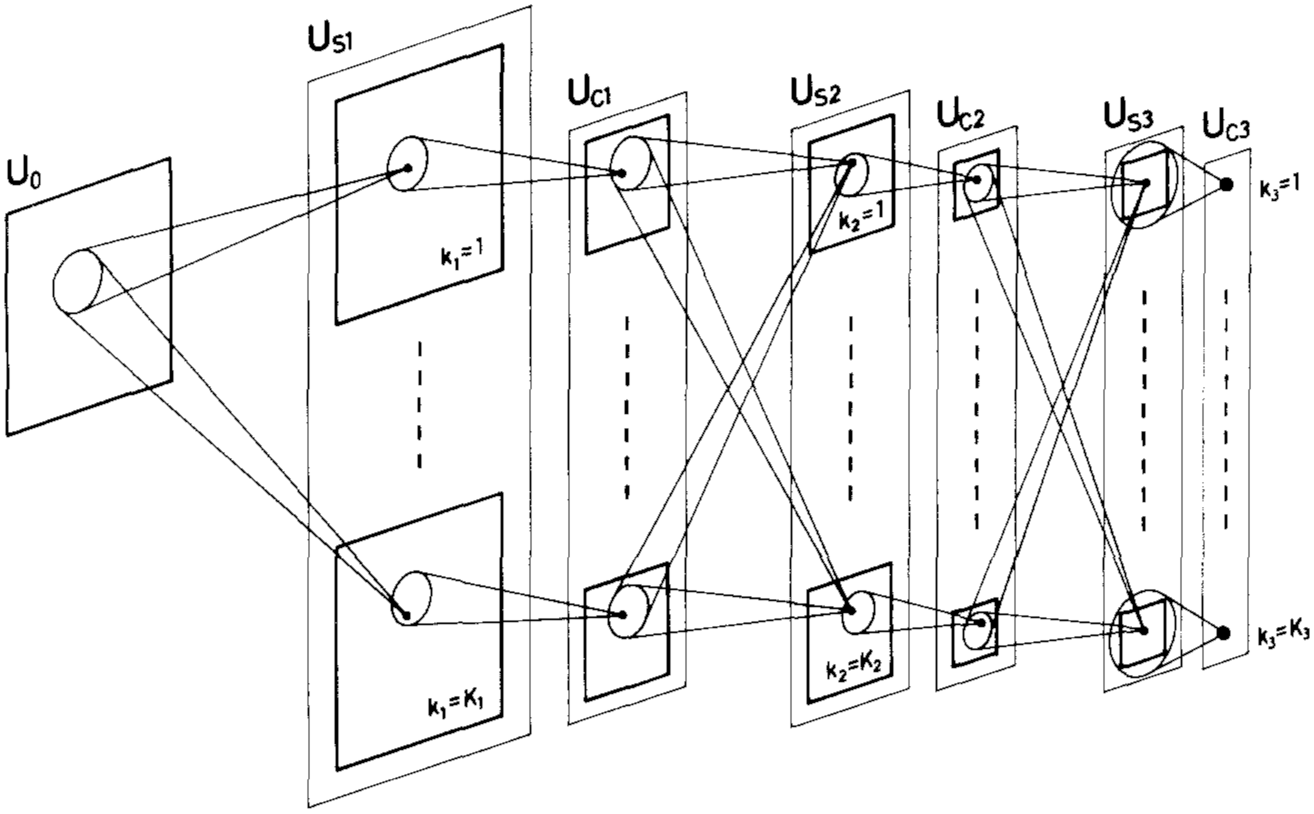
\includegraphics[width=0.8\textwidth]{cover.png}
\end{figure}

\vspace*{\stretch{1}}

\footnotesize \dotdate\today

\end{center}

\newpage

%%%%%%%%%%%%%%%%%%%%%%%%%%%%%%%%%%%%%%%%%%%%%%%%%%%%%%%%%%%%%%%%%%%%%%%%%%%%%%%%%%%%%%%%%%%

\vspace*{\stretch{1.25}}

\href{https://fleuret.org/francois/}{François Fleuret} 是瑞士日内瓦大学计算机科学教授。

封面插图是新认知机(Neocognitron) 的示意图,来自 Fukushima [1980],它是深度神经网络的重要前身。

本书格式适配手机屏幕。

\vspace*{\stretch{1}}

\vspace*{-3ex}

\newpage

%%%%%%%%%%%%%%%%%%%%%%%%%%%%%%%%%%%%%%%%%%%%%%%%%%%%%%%%%%%%%%%%%%%%%%%%%%%%%%%%%%%%%%%%%%%
% Table of content
%%%%%%%%%%%%%%%%%%%%%%%%%%%%%%%%%%%%%%%%%%%%%%%%%%%%%%%%%%%%%%%%%%%%%%%%%%%%%%%%%%%%%%%%%%%

{
\everymath{\color{black}}
\tableofcontents % Prints the table of contents
%\addcontentsline{toc}{chapter}{Contents}
}

\clearpage

\listoffigures*
\addcontentsline{toc}{chapter}{插图列表}

%%%%%%%%%%%%%%%%%%%%%%%%%%%%%%%%%%%%%%%%%%%%%%%%%%%%%%%%%%%%%%%%%%%%%%%%%%%%%%%%%%%%%%%%%%%

\chapter*{前言}
\addcontentsline{toc}{chapter}{前言}

\citep{nips-1502.c399862d3b9d6b76c8436e924a68c45b} 证明,仅用二十多年前[\cite[LeCun et al., 1989]{lecun-89e}]诞生的结构简单的\emph{人工神经网络},只需放大百倍,并在同等放大的数据集上进行训练,就可以以巨大优势击败当时最先进的复杂图像识别方法。这一发现引发了当今人工智能的进步。

这一突破得益于\emph{图形处理单元} (\emph{GPU})、大众市场以及原本为实时图像合成而开发现在重新应用于人工神经网络的高度并行计算设备。

从那时起,在``\emph{深度学习}''这一总称下,各种网络结构、训练策略和专用硬件的创新使得人工神经网络的规模和训练所用数据量呈指数级增长 [\ref{}{Sevilla et al., 2022}]。这掀起了从计算机视觉与机器人科学到语音和自然语言处理等一系列技术领域的成功应用浪潮。

尽管深度学习的大部分内容并不难理解,但它综合了线性代数、微积分、概率、优化、信号处理、编程、算法和高性能计算等不同的学科知识,使得学习变得复杂。

这本小书不会试图详尽无遗,而是仅限于理解重要模型所需的背景知识。事实证明,这是一种广受好评的方法,本书在 Twitter 上发布一个月内,PDF 版本的下载量就达到了 25 万次。

如果您没有从官网 
\begin{center}
\href{https://fleuret.org/public/lbdl.pdf}{https://fleuret.org/public/lbdl.pdf}
\end{center}
获取本书,请从官网下载,以便我可以统计读者的数量。

\begin{flushright}
  François Fleuret,\\
  2023.06.23
\end{flushright}

%%%%%%%%%%%%%%%%%%%%%%%%%%%%%%%%%%%%%%%%%%%%%%%%%%%%%%%%%%%%%%%%%%%%%%%%%%%%%%%%%%%%%%%%%%%

\part{基础}

% !TeX root = ../main.tex
\chapter{机器学习}
% !TeX root = ../main.tex
\chapter{高性能计算}

从实现的角度来看,深度学习涉及使用大量数据执行繁重的计算。\keyterm{图形处理单元} (\keyterm{GPU}) 可以在经济实惠的硬件上运行此类计算,从而对该领域的成功发挥了至关重要的作用。

使用 GPU 的重要性,以及由此产生的对有效计算的技术限制,迫使该领域的研究不断平衡数学的合理性和新方法的可实施性。

\section{GPU、TPU 和批处理}

图形处理单元最初是为实时图像合成而设计的,这需要高度并行的架构,而这种架构恰好非常适合深度模型。随着人工智能用途的增加,GPU 配备了专用的\keyterm{张量核心},并且开发了深度学习专用芯片,例如谷歌的\keyterm{张量处理单元}(\keyterm{TPU})。

GPU 拥有数千个并行单元和自己的快速内存。限制因素通常不是计算单元的数量,而是\keyterm{对内存的读写操作}。最慢的链接位于 CPU 内存和 GPU 内存之间,因此应避免跨设备复制数据。此外,GPU 本身的结构涉及多级\keyterm{缓存},这些缓存容量更小但速度更快,并且应该组织计算以避免不同缓存之间的复制。

具体来说,就是通过将计算组织为完全适合 GPU 内存的\keyterm{样本批次}再通过并行处理来实现的。当操作器组合样本和模型参数时,两者都必须移动到实际计算单元附近的高速缓存中。分批进行仅允许复制模型参数一次,而不是为每个样本复制一次。实际上,GPU 处理适合内存的批次几乎与处理单个样本一样快。

标准 GPU 的理论\keyterm{峰值性能}为每秒 $10^{13}-10^{14}$ 次浮点运算 (\keyterm{FLOP}),其内存通常在 $8$ 到 $80$ GB 之间。标准 \keyterm{FP32} 采用 $32$ 位编码浮点数,但经验结果表明,使用 $16$ 位编码,甚至对某些操作数采用更低的编码,不会降低性能。

我们将在 \ref{sec3.7} 节中讨论深度架构的尺寸。

\section{张量}

GPU 与 PyTorch 或 JAX 等\keyterm{深度学习框架}通过将要处理的量组织为\keyterm{张量}来操作要处理的量,张量是沿多个离散轴排列的一系列标量。它们是 $\mathbb{R}^{N_1 \times \dots \times N_D}$ 的元素,泛化了向量和矩阵的概念。

张量用于表示要处理的信号、模型的\keyterm{可训练参数}以及它们计算的中间量。后者被称为\keyterm{激活},指的是神经元激活。

例如,时间序列自然地被编码为 $T \times D$ 张量,或者,由于历史原因,编码为 $D \times T$ 张量,其中 $T$ 是其持续时间,$D$ 是每个时间帧特征表示的维度,通常称为\keyterm{通道}数。类似地,二维结构信号可以表示为 $D \times H \times W$ 张量,其中 $H$ 和 $W$ 是其高度和宽度。RGB 图像对应于 $D = 3$,但在大型模型中通道数可能会多至到数千个。

添加更多维度可以表示一系列对象。例如,$50$ 个分辨率为 $32 \times 24$ 的 RGB 图像可以编码为 $50 \times 3 \times 24 \times 32$ 张量。

深度学习库提供了大量操作,包括标准线性代数、复杂重塑和提取以及深度学习特定操作,其中一些我们将在第 \ref{ch4} 章中看到。张量的实现将形状表示与内存中系数的存储布局分开。这允许在不复制系数的情况下完成许多重塑、转置和提取操作,因此速度非常快。

在实践中,几乎任何计算都可以分解为基本张量运算,这避免了语言级别的非并行循环和不良的内存管理。

除了方便使用之外,张量还有助于提高计算效率。所有参与开发可操作深度模型的人员,从驱动程序、库和模型的设计者到计算机和芯片的设计者,都知道数据将作为张量进行操作。由此产生的对局部性和块可分解性的限制使该链条中的所有参与者都能给出最佳设计。
% !TeX root = ../main.tex
\chapter{训练}

如 \ref{sec1.1} 节所述,训练模型包括最小化损失 $\mathcal{L}(w)$,它反映了预测器 $f(\cdot;w)$ 在\keyterm{训练集} $\mathcal{D}$ 上的表现。

由于模型通常非常复杂,并且其表现与损失最小化程度直接相关,因此这里的最小化是一个关键挑战,涉及计算和数学难题。

\section{损失}

公式 \ref{eq1.1} 中的\keyterm{均方误差}示例是用于预测连续值的标准损失。

在密度建模中,标准损失是数据的似然度。如果 $f(x;w)$ 被解释为归一化的对数概率或对数密度,那么损失就是其值在训练样本上的总和的相反数,这对应于数据集的似然度。

\subsubsection*{交叉熵}

对于\keyterm{分类},通常的策略是模型的输出是一个向量,其中每个类别 $y$ 对应一个分量 $f(x;w)_y$,这被解释为非归一化概率的对数或 \keyterm{logit}。

如果 $X$ 为输入信号,$Y$ 为要预测的类别,我们可以根据 $f$ 计算\keyterm{后验概率}估计:
\[\hat{P}(Y=y \mid X=x) = \frac{\exp f(x;w)_y}{\sum_{z}\exp f(x;w)_z}\]
该表达式通常称为 logits 的 \keyterm{softmax},或更准确地说,称为 \keyterm{softargmax}。

为了与这种解释保持一致,模型应该被训练来最大化真实类别的概率,因此要最小化交叉熵,其表达式如下:
\begin{align*}
    \mathcal{L}_{ce}(w) &= -\frac{1}{N}\sum_{n=1}^{N} \log \hat{P}(Y=y_n \mid X=x_n) \\
    &= \frac{1}{N}\sum_{n=1}^{N} \underbrace{-\log \frac{\exp f(x_n;w)_{y_n}}{\sum_{z}\exp f(x_n;w)_z}}_{L_{ce}(f(x_n;w),y_n)}
\end{align*}

\subsubsection*{对比损失}

在某些设置中,即使要预测的值是连续的,监督也会采取排名约束的形式。这种情况的典型领域是\keyterm{度量学习},其目标是学习样本之间距离的度量,使得来自某个语义类别的样本 $x_a$ 与同一类别中的任意样本 $x_b$ 之间的距离都比来自另一个类别的任意样本 $x_c$ 之间的距离更近。例如,$x_a$ 和 $x_b$ 可以是某个人的两张照片,而 $x_c$ 则是另一个人的照片。

这种情况的标准方法是最小化\keyterm{对比损失},在这种情况下,例如,三元组 $(x_a,x_b,x_c)$,满足 $y_a = y_b \ne y_c$,求和
\[\max(0,1-f(x_a,x_c;w)+f(x_a,x_b;w))\]
除非 $f(x_a,x_c;w) \ge 1+f(x_a,x_b;w)$,否则该量将严格为正。

\subsubsection*{工程化损失}

通常,在训练期间最小化的损失并不是最终想要优化的实际量,而是一个代理量,是为了让找到最佳模型参数更为容易。例如,尽管实际的性能度量是分类错误率,但交叉熵是分类的标准损失,因为后者没有提供信息梯度,这是我们将在 \ref{sec3.3} 节中看到的关键要求。

还可以在损失中添加取决于模型本身的可训练参数项,以支持某些配置。

例如,\keyterm{权重衰减}正则化包括向损失中增加一个与参数平方和成比例的项。这可以被解释为在参数上施加了一个高斯贝叶斯先验,它偏好较小的值,从而减少了数据的影响。这会降低其在训练集上的表现,但会减少训练表现与新的、未见过的数据上的表现之间的差距。

\section{自回归模型}

自回归模型是一类关键方法,特别适用于处理自然语言处理和计算机视觉中的离散序列。

\subsubsection*{概率的链式法则}

这些模型使用概率论中的\keyterm{链式法则}:
\begin{align*}
    P(&X_1 = x_1,X_2 = x_2,\dots,X_T = x_T) = \\
    &P(X_1 = x_1) \\
    \times &P(X_2 = x_2 \mid X_1 = x_1) \\
    &\dots \\
    \times &P(X_T = x_T \mid X_1 = x_1,\dots,X_{T-1} = x_{T-1})
\end{align*}
尽管这种分解对于任何类型的随机序列都有效,但当感兴趣的信号是来自有限\keyterm{词汇表} $\{1, \dots ,K\}$ 的 \keyterm{Token} 序列时,它特别有效。

按照约定,附加 Token $\emptyset$ 代表``未知''量,我们可以将事件 ${X_1 = x_1,\dots,X_t = x_t}$ 表示为向量 $(x_1,\dots,x_t,\emptyset,\dots,\emptyset)$。则模型
\[f : \{\emptyset,1,\dots,K\}^T \to \mathbb{R}^K\]
在给定这样的输入的情况下计算与
\[\hat{P}(X_t \mid X_1 = x_1,\dots,X_{t-1} = x_{t-1})\]
相对应的 $K$ 个 \keyterm{logits} 的向量 $l_t$,允许在给定先前 Token 的情况下对一个 Token 进行采样。

链式法则确保在给定先前采样的 $x_1,\dots,x_{t-1}$ 的情况下,通过一次次地对第 $T$ 个 Token $x_t$ 进行采样,我们能够得到一个遵循联合分布的序列。这是一个\keyterm{自回归}生成模型。

训练这样的模型可以通过最小化训练序列和时间帧上的\keyterm{交叉熵损失}
\[Lce\big(f(x_1,\dots,x_{t-1},\emptyset,\dots,\emptyset;w),x_t\big)\]
之和来完成,这在形式上等同于最大化真实 $x_t$ 的似然。

传统上监测的值不是交叉熵本身,而是\keyterm[困惑度]{困惑度(Perplexity)},其定义为交叉熵的指数。它对应于具有相同熵的均匀分布的值的数量,这通常更易于解释。

\subsubsection*{因果模型}

我们所描述的训练过程对于每个 $t$ 都需要不同的输入,而且在 $t < t'$ 的情况下所做的大部分计算会在 $t'$ 时重复进行。这是极其低效的,因为 $T$ 通常是几百或几千的数量级。

解决这个问题的标准策略是设计一个模型 $f$ 一次性预测所有 logits 向量 $l_1,\dots,l_T$,即:
\[f : {1,\dots,K}^T \to \mathbb{R}^{T \times K}\]
但存在计算结构使得计算 $x_t$ 的 logits $l_t$ 仅依赖于输入值 $x_1,\dots,x_{t-1}$。

\begin{figure}
    \centering
    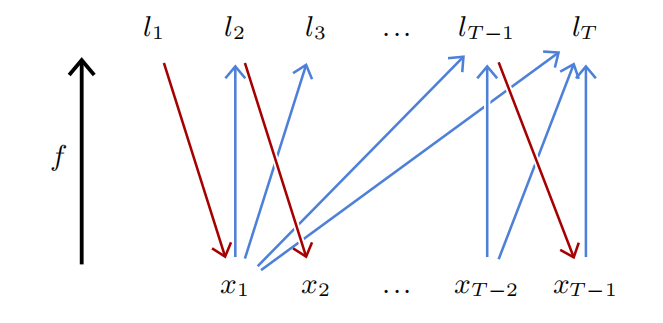
\includegraphics[width=0.9\textwidth]{fig/fig3.1.png}
    \caption[因果自回归模型]{如果输入序列的一个时间帧 $x_t$ 调节预测的 logits $l_s$ 只在 $s > t$ 时才有效,如蓝色箭头所示,则自回归模型 $f$ 是因果模型。这允许在训练期间一次性计算所有时间帧的分布。然而,在采样过程中,$l_t$ 和 $x_t$ 是顺序计算的,后者是用前者采样的,如红色箭头所示。}
    \label{fig3.1}
\end{figure}

这样的模型称为\keyterm{因果模型},因为在时间序列的情况下,它对应于不让未来影响过去,如图 \ref{fig3.1} 所示。

其结果是,每个位置上的输出都假设输入只在该位置之前可用的情况下所得到的。在训练过程中,这使得我们能够计算一个完整序列的输出,并最大化该序列所有 token 的预测概率,这又归结为最小化每个 token 的交叉熵之和。

请注意,为了简单起见,我们将 $f$ 定义为对长度固定为 $T$ 的序列进行操作。然而,实际使用的模型,例如我们将在 \ref{sec5.3} 节中看到的 Transformer 模型,能够处理任意长度的序列。

\subsubsection*{分词器(Tokenizer)}

处理自然语言时,一个重要技术细节是,token 的表示方法多种多样,从最细粒度的单个符号到整个单词,不一而足。而 token 表示的转换是由一个称为\keyterm{分词器}(\keyterm{tokenizer})的独立算法来完成的。

一种标准的方法是\keyterm{字节对编码}(\keyterm{Byte Pair Encoding},\keyterm{BPE})\citep{srivastava14a},它通过分层合并字符组来构造 token,尝试获取代表不同长度但频率相似的单词片段的 token,并将 token 分配给长的高频片段以及罕见的单个符号。

\section{梯度下降}\label{sec3.3}

除了在 \ref{sec1.2} 节中看到的线性回归等特定情况外,最优参数 $w^*$ 没有闭合形式的表达式。在一般情况下,最小化函数的选择工具是\keyterm{梯度下降}。它首先使用随机值 $w_0$ 初始化参数,然后通过迭代\keyterm{梯度步骤}来改进该估计,每个梯度步骤包括计算损失相对于参数的梯度,并减去其中的一小部分:
\begin{equation}
    w_{n+1} = w_n - \eta \nabla \mathcal{L}_{\mid w}(w_n)\label{eq3.1}
\end{equation}
此过程相当于将当前估计值超微朝局部最优方向最大化地减小 $\mathcal{L}(w)$,如图 \ref{fig3.2} 所示。

\begin{figure}
    \centering
    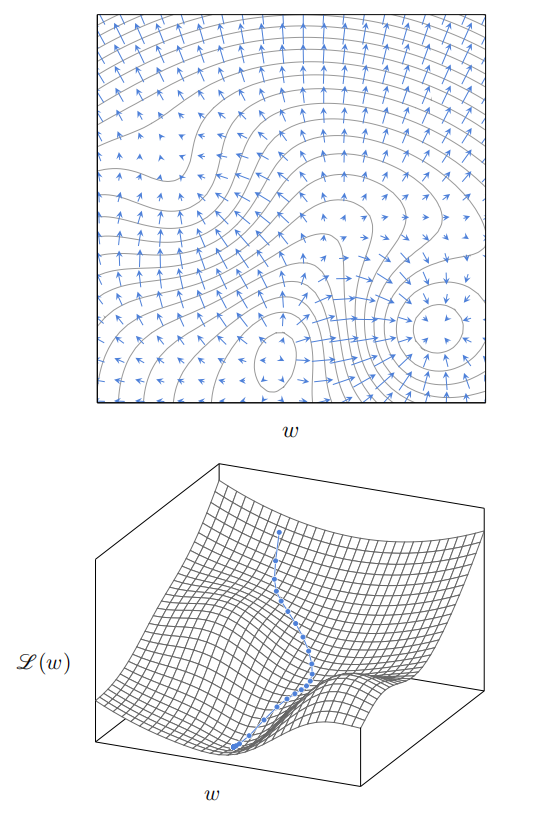
\includegraphics[width=0.9\textwidth]{fig/fig3.2.png}
    \caption[梯度下降]{对于每个点 $w$,梯度 $\nabla \mathcal{L}_{\mid w}(w)$ 都处于使 $\mathcal{L}$ 增加最大化的方向,与水平曲线(上图)正交。梯度下降通过在每一步减去梯度的一小部分来迭代地最小化 $\mathcal{L}(w)$,从而产生遵循最陡下降的轨迹(下图)。}
    \label{fig3.2}
\end{figure}

\subsubsection*{学习率}

\keyterm{元参数} $\eta$ 称为\keyterm{学习率}。它是一个正值,可调节最小化完成的速度,必须谨慎选择。

如果该值太小,优化会很慢,并可能会过早陷入局部最小值。如果该值太大,优化可能会在某个最小值附近反复跳动,从而永远无法下降到该最小值。正如我们将在 \ref{sec3.6} 节中看到的,学习率可以依据迭代次数 $n$ 来调节。

\subsubsection*{随机梯度下降}

实际中使用的所有损失都可以表示为每一小组样本或每个样本的平均损失,例如:
\[\mathcal{L}(w) = \frac{1}{N} \sum_{n=1}^{N} \mathcal{l}_n(w)\]
其中对于某个 $L$,$\mathcal{l}_n(w) = L(f(x_n;w),yn) f$,那么梯度可以表示为
\begin{equation}
    \nabla \mathcal{L}_{\mid w}(w) = \frac{1}{N} \sum_{n=1}^{N} \nabla \mathcal{l}_{n \mid w}(w)\label{eq3.2}
\end{equation}
尽管通常来说这里地计算量很大,由此产生的\keyterm{梯度下降}将精确计算公式 \ref{eq3.2} 中的求和,然后根据公式 \ref{eq3.1} 更新参数。然而,在合理的可交换性假设下,例如,如果样本已被适当地随机打乱,则方程 \ref{eq3.2} 的任何部分之和都是总和的无偏估计,尽管这样做会带来噪声。因此,从部分之和更新参数相当于在相同计算预算下执行更多的梯度步骤,并且梯度估计的噪声更大。由于数据的冗余,这恰好是一种更有效的策略。

我们在 \ref{sec2.1} 节中看到,处理一批大小适合计算设备内存的样本通常与处理单个样本一样快。因此,标准方法是将全集 $\mathcal{D}$ 分成\keyterm{批次},并根据每个批次计算的梯度估计来更新参数。这称为小批次随机梯度下降,简称\keyterm{随机梯度下降}(\keyterm{SGD})。

需要注意的是,这一过程是极其缓慢的,小批次数据和梯度步骤的数量通常达到数百万的量级。

与许多算法一样,直觉在高维中会崩溃,尽管看起来这个过程很容易陷入局部最小值,但实际上,由于参数数量、模型设计和数据的随机性,其效率远远高于人们的预期。

人们已经提出了许多该标准策略的变体。其中最流行的是 \citep{arxiv-1412.6980},它可以进一步对每个梯度分量的平均值和方差进行估算,并自动将其归一化,避免了缩放问题以及模型不同部分训练速度不一致问题。

\section{反向传播}

\subsubsection*{正向和反向传递}

\subsubsection*{资源利用}

\subsubsection*{梯度消失}

\section{深度值}\label{sec3.6}

\section{训练协议}\label{sec3.7}

\section{规模的好处}

%%%%%%%%%%%%%%%%%%%%%%%%%%%%%%%%%%%%%%%%%%%%%%%%%%%%%%%%%%%%%%%%%%%%%%%%%%%%%%%%%%%%%%%%%%%

\part{深度模型}

% !TeX root = ../main.tex
\chapter{模型构成}\label{ch4}

深度模型只不过是复杂的张量计算,最终可以用线性代数和数学分析分解为标准数学运算。多年来,该领域开发了大量语义清晰的高级模块以及由这些模块组合而来的复杂模型,这些模型已被证明在特定应用领域非常有效。

经验证据和理论结果表明,更深的架构(即长映射组合)可以获得更好的表现。正如我们在 \ref{sec3.4} 节中看到的,由于\keyterm{梯度消失},训练这样的模型具有挑战性,而多项重要技术贡献缓解了这个问题。

\section{层的概念}\label{sec4.1}

我们将那些被设计出来并通过经验认定为通用且高效的标准复杂复合张量操作称为\keyterm{层}。这些层通常包含可训练参数,并且对于设计和描述大型深度模型来说,它们提供了一个便捷的粒度级别。这个术语来源于简单多层神经网络,尽管现代模型可能采用此类模块的复杂图形形式,并包括多个并行路径。

\begin{figure}[h]
    \centering
    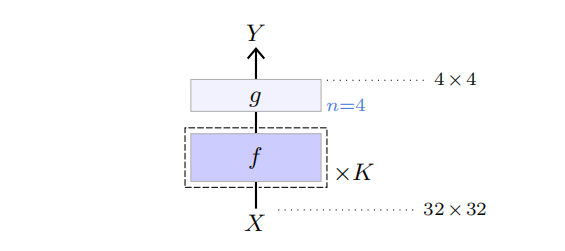
\includegraphics[width=0.9\textwidth]{fig/fig4.0.png}
\end{figure}

在接下来的几页中,我将遵循上面所示模型绘制的约定:

\begin{itemize}
    \item 运算符/层被绘制为框,
    \item 深色表示嵌入了可训练的参数,
    \item 没有默认值的元参数用蓝色字添加在右侧,
    \item 带有乘法因子的虚线外框表示一组层按顺序复制,每个层都有自己的一组可训练参数(如果有的话),
    \item 在某些情况下,当输出维度与输入维度不同时,会在右侧标明。
\end{itemize}

此外,具有复杂内部结构的层会用高度更高的框来表示。

\section{线性层}\label{sec4.2}

就计算和参数数量而言,最重要的模块是\keyterm{线性层}。它们得益于数十年来在矩阵运算算法和芯片设计方面的研究与工程进步。

请注意,在深度学习中,``线性''这一术语通常不恰当地指代\keyterm{仿射运算},即一个线性表达式和一个常数偏置之和。

\subsubsection*{全连接层}

最基本的线性层是\keyterm{全连接层},由大小为 $D' \times D$ 的可训练权重矩阵 $W$ 和维度为 $D'$ 的偏置向量 $b$ 参数化。它实现了泛化到任意张量形状的仿射变换,其中补充的维度被解释为向量索引。形式上,给定维度为 $D_1 \times \dots \times D_K \times D$ 的输入 $X$,它计算出维度为 $D_1 \times \dots \times D_K \times D'$ 的输出 $Y$,其中
\begin{align*}
    \forall d_1,\dots,d_K&,\\
    Y[d_1&,\dots,d_K] = WX[d_1,\dots,d_K]+b
\end{align*}
虽然乍看之下,这种仿射运算似乎仅限于旋转、对称和平移等几何变换,但实际上它能做的远不止这些。特别是,用于降维或信号过滤的投影,而且,从点积作为相似性度量的角度来看,矩阵-向量乘积可以解释为计算输入向量所编码的查询与矩阵行所编码的键之间的匹配得分。

正如我们在 \ref{sec3.3} 节中看到的,梯度下降从\keyterm{参数的随机初始化}开始。如果这一操作做得过于简单,如 \ref{sec3.4} 节所示,网络可能会遭受激活和梯度爆炸或消失的影响 \citep{glorot10a}。深度学习框架实现了初始化方法,特别是按照输入的维度来缩放随机参数,以保持激活的方差恒定并防止病态行为。

\subsubsection*{卷积层}

线性层可以将任意形状的张量通过重塑成向量的方式作为输入,只要它具有正确数量的系数即可。然而,这样的层不太适合处理大型张量,因为参数数量和操作数量与输入和输出维度的乘积成正比。例如,要处理一个大小为 $256 \times 256$ 的 RGB 图像作为输入并计算相同大小的结果,将需要大约 $4 \times 10^{10}$ 个参数和乘法运算。

除了这些实际问题之外,大多数高维信号都是强结构化的。例如,图像在平移、缩放和某些对称性方面表现出短期相关性和统计平稳性。这并没有反映在全连接层的\keyterm{归纳偏置}中,它完全忽略了信号结构。

为了利用这些规律,首选的工具是\keyterm{卷积层}。卷积层同样是仿射的,但它局部处理时间序列或二维信号,并在各处使用相同的操作符。

\keyterm{一维卷积}主要由三个\keyterm{元参数}定义:内核大小 $K$、输入通道数 $D$、输出通道数 $D'$,以及仿射映射 $\phi(\cdot;w):\mathbb{R}^{D \times K} \to \mathbb{R}^{D' \times 1}$ 的可训练参数 $w$。

它可以处理任何大小为 $D \times T$ 且 $T \ge K$ 的张量 $X$,并将 $\phi(\cdot;w)$ 应用于 $X$ 的每个大小为 $D \times K$ 的子张量,将结果存储在大小为 $D' \times (T-K+1)$ 的张量 $Y$ 中,如图 \ref{fig4.1}(左半部分)所示。

\newpage

\begin{figure}[h]
    \centering
    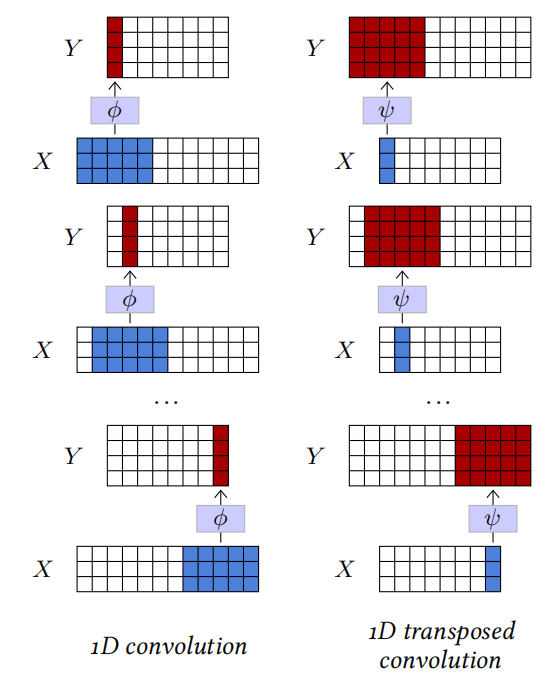
\includegraphics[width=0.9\textwidth]{fig/fig4.1.png}
    \caption[一维卷积]{一维卷积(左)接受 $D \times T$ 张量 $X$ 作为输入,将相同的仿射映射 $\phi(\cdot;w)$ 应用于形状为 $D \times K$ 的每个子张量,并将生成的 $D' \times 1$ 张量存储到 $Y$ 中。一维转置卷积(右)接受 $D \times T$ 张量作为输入,将相同的仿射映射 $\phi(\cdot;w)$ 应用于每个形状为 $D \times 1$ 的子张量,并对偏移后的 $D' \times K$ 结果张量求和。两者都可以处理不同大小的输入。}
    \label{fig4.1}
\end{figure}

\keyterm{二维卷积}与之类似,但具有 $K \times L$ 大小的内核,并接受 $D \times H \times W$ 大小的张量作为输入(参见图 \ref{fig4.2},左半部分)。

\begin{figure}[h]
    \centering
    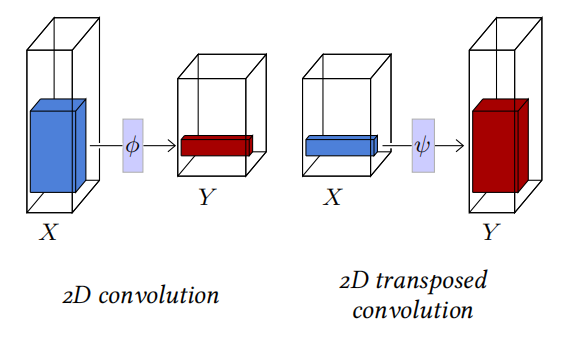
\includegraphics[width=0.9\textwidth]{fig/fig4.2.png}
    \caption[二维卷积]{二维卷积(左)接受 $D \times H \times W$ 张量 $X$ 作为输入,将相同的仿射映射 $\phi(\cdot;w)$ 应用于形状为 $D \times K \times L$ 的每个子张量,并将生成的 $D' \times 1 \times 1$ 张量存储到 $Y$ 中。二维 转置卷积(右)接受 $D \times H \times W$ 张量作为输入,将相同的仿射映射 $\phi(\cdot;w)$ 应用于每个形状为 $D \times 1 \times 1$ 的子张量,并对偏移后的 $D' \times K \times L$ 结果张量求和得到 $Y$。}
    \label{fig4.2}
\end{figure}



这两种操作的可训练参数都是 $\phi$ 的参数,可以分别将其设想为大小为 $D \times K$ 或 $D \times K \times L$ 的 $D'$ 个\keyterm{过滤器},以及一个维度为 $D'$ 的\keyterm{偏置向量}。

这样的层对平移是\keyterm{等变}的,这意味着如果输入信号被平移,输出也会以类似的方式变换。当处理其分布对于平移不变的信号时,此属性会产生理想的\keyterm{归纳偏差}。

卷积层还接受三个额外的\keyterm{元参数},如图 \ref{fig4.3} 所示:

\begin{itemize}
    \item \keyterm{填充}指定在处理输入张量之前应在输入张量周围添加多少个零系数,特别是在内核大小大于 $1$ 时维持张量尺寸。其默认值为 $0$。
    \item \keyterm{步幅}指定在处理输入时使用的步长,允许通过使用大步长以几何方式减小输出大小。其默认值为 $1$。
    \item \keyterm{膨胀}指定局部仿射操作符的过滤器系数之间的索引计数。其默认值为 $1$,更大的值对应于在系数之间插入零,这会增加过滤器/内核的大小,同时保持可训练参数数量不变。
\end{itemize}

\begin{figure}
    \centering
    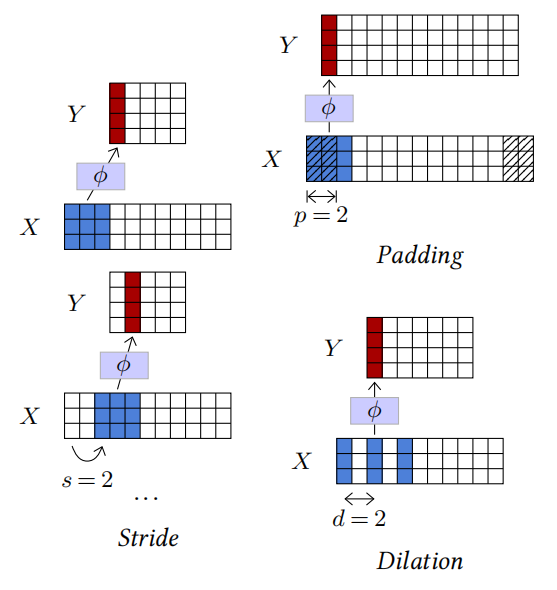
\includegraphics[width=0.9\textwidth]{fig/fig4.3.png}
    \caption[步长、填充和膨胀]{除了内核大小和输入/输出通道数之外,卷积还接受三个元参数:步长 $s$(左)在经过输入张量时调节步长,填充 $p$(右上)指定在处理输入张量之前在输入张量周围添加多少个零元素,膨胀 $d$(右下)参数化过滤器系数之间的索引计数。}
    \label{fig4.3}
\end{figure}

除了通道数之外,卷积的输出通常小于其输入。在没有填充或膨胀的一维情况下,如果输入的大小为 $T$,内核的大小为 $K$,步幅为 $S$,则输出的大小为 $T' = (T - K)/S + 1$。

\newpage

给定由卷积层计算的激活,或某个位置上所有通道的值向量,它所依赖的输入信号部分称为其\keyterm{感受野}(见图 \ref{fig4.4})。与 $D \times H \times W$ 激活张量的单个通道对应的 $H \times W$ 子张量之一称为\keyterm{激活图}。

\begin{figure}
    \centering
    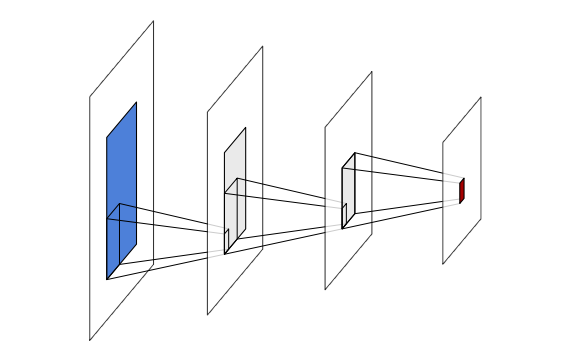
\includegraphics[width=0.9\textwidth]{fig/fig4.4.png}
    \caption[感受野]{给定一系列卷积层(这里为红色)中的激活,其\keyterm{感受野}是输入信号(蓝色)中调节其值的区域。每个中间卷积层大约按照核的宽度和高度增加该区域的宽度和高度。}
    \label{fig4.4}
\end{figure}

卷积用于重新组合信息,通常是为了减少表示的空间大小,以换取更多数量的通道,从而转化为更丰富的局部表示。它们可以实现微分运算符,例如边缘检测器或模板匹配机制。一系列这样的层也可以视为一种组合和分层表示 \citep{arxiv-1311.2901},或者作为一个扩散过程,其中信息在穿过层时可以通过内核大小的一半进行传输。

逆运算是\keyterm{转置卷积},也由局部仿射运算符组成,由与卷积类似的元和可训练参数定义,例如,在一维情况下,它将一个仿射映射 $\phi(\cdot;w):R^{D \times 1} \to R^{D' \times K}$ 应用于输入的每个 $D \times 1$ 子张量,并将偏移后的 $D' \times K$ 结果张量求和以计算其输出。这样的操作符增加了信号的尺寸,直观上可以理解为一个合成过程(见图 \ref{fig4.1} 和图 \ref{fig4.2} 的右半部分)。

一系列卷积层是将大维度信号(如图像或声音样本)映射到低维张量的常用架构。例如,这可以用来获取用于分类的类别分数或压缩表示。转置卷积层以相反的方式用来从压缩表示构建大维度信号,要么是为了评估压缩表示是否包含足够的信息来重构信号,要么是为了合成,因为在低维表示上学习密度模型更容易。我们将在 \ref{sec5.2} 节中重新讨论这个话题。

\section{激活函数}\label{sec4.3}

如果网络仅组合线性组件,那么它本身就只是线性运算符,因此让网络具有非线性运算非常必要。这些\keyterm{非线性运算}主要是通过\keyterm{激活函数}来实现的,激活函数是将输入张量的每个分量单独通过一个映射进行转换的层,从而得到一个相同形状的张量。

有许多不同的激活函数,但最常用的是\keyterm{线性整流函数}(\keyterm{ReLU}) \citep{glorot11a},它将负值设置为零并保持正值不变(见图 \ref{fig4.5},右上)
$$
\text{relu}(x) = \begin{cases}
    0 &\text{如果}\; x < 0 \\
    x &\text{如果}\; x \ge 0
 \end{cases}
 $$
 鉴于深度学习的核心训练策略依赖于梯度,因此一个在零点不可微且在数轴正半轴为常数的映射似乎是有问题的。然而,梯度下降所需的主要属性是梯度平均具有信息性。训练开始时,参数初始化和数据归一化使一半的激活为正,从而确保了这一点。

 \begin{figure}
    \centering
    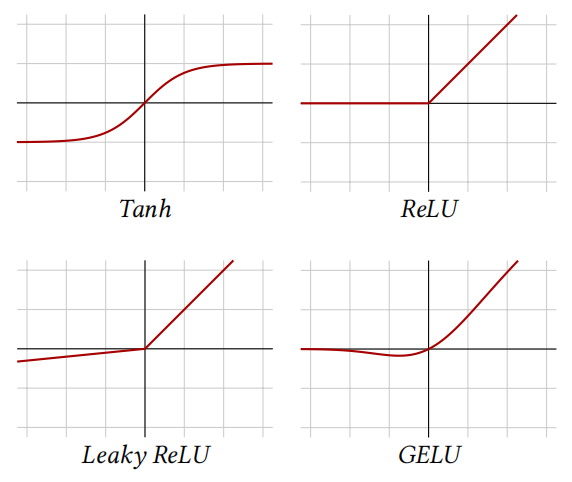
\includegraphics[width=0.9\textwidth]{fig/fig4.5.png}
    \caption[激活函数]{激活函数。}
    \label{fig4.5}
\end{figure}

在 ReLU 被普遍使用之前,标准激活函数是\keyterm{双曲正切函数}(\keyterm{Tanh},见图 \ref{fig4.5},左上),它在负半轴和正半轴都会以指数速度快速饱和,这加剧了梯度消失。

其他流行的激活函数遵循相同的思路,即保持正值不变压缩负值。\keyterm{Leaky ReLU} \citep{relu_hybrid_icml2013_final} 对负值应用一个小的正乘法因子(见图 \ref{fig4.5},左下):
$$
\text{leakyrelu}(x) = \begin{cases}
    ax &\text{如果}\; x < 0 \\
    \enspace x &\text{如果}\; x \ge 0
 \end{cases}
 $$
 而 \keyterm{GELU} \citep{arxiv-1606.08415} 是利用高斯分布的累积分布函数来定义的,即:
 \[\text{gelu}(x) = xP(Z \le x)\]
 其中 $Z \sim \mathcal{N} (0,1)$。它的行为大致类似于平滑的 ReLU(见图 \ref{fig4.5},右下)。

 激活函数的选择,特别是 ReLU 变体的选择,通常是由经验表现驱动的。

\section{池化}\label{sec4.4}

减少信号大小的一种经典策略是使用\keyterm{池化}操作,将多个激活合并为一个理想情况下能总结信息的激活。此类操作中最标准的是\keyterm{最大池化}层,它与卷积类似,可以在一维和二维中操作,并由\keyterm{内核大小}定义。

在其标准形式中,该层在空间大小等于内核大小的非重叠子张量上计算每个通道的最大激活。这些值存储在与输入具有相同通道数的结果张量中,并且其空间大小能被内核大小整除。与卷积一样,该运算符具有三个\keyterm{元参数}:\keyterm{填充}、\keyterm{步长}和\keyterm{膨胀},默认情况下步长等于内核大小。遵循与卷积相同的公式(参见第 \ref{sec4.2} 节),较小的步长会产生较大的结果张量。

最大操作可以直观地解释为逻辑析取,或者,当它经过一系列通过计算局部分数来表示部件存在的\keyterm{卷积层}时,作为一种编码方式编码至少有一个部件实例存在。它牺牲了精确位置,从而使其不受局部变形的影响。

一个常见的替代方案是\keyterm{平均池化}层,它计算子张量上的平均值而不是最大值。这是一种线性操作,而最大池化则不是。

\begin{figure}
    \centering
    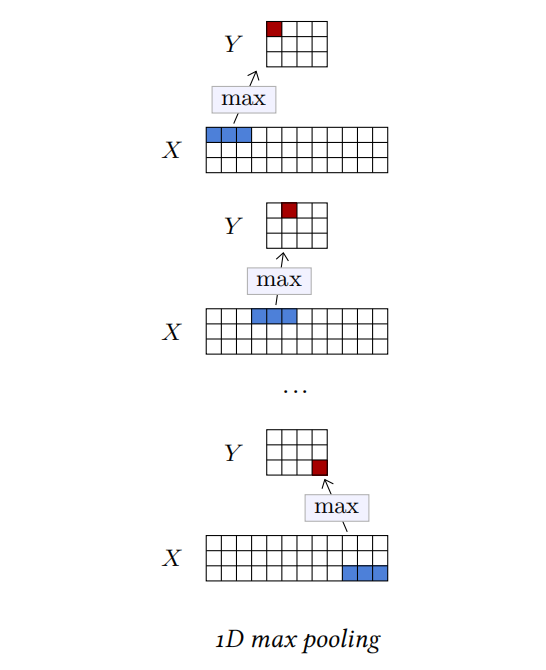
\includegraphics[width=0.9\textwidth]{fig/fig4.6.png}
    \caption[最大池化]{一维最大池化将 $D \times T$ 大小的张量 $X$ 作为输入,计算非重叠 $1 \times L$ 子张量(蓝色)的最大值,并将结果值(红色)存储在 $D \times (T / L)$ 大小的张量 $Y$ 中。}
    \label{fig4.6}
\end{figure}

\section{Dropout}\label{sec4.5}

某些层被专门设计用来促进训练或改进学学习得到的表示。

这类主要贡献之一是 \keyterm{Dropout} \citep{srivastava14a}。这种层没有可训练参数,但有一个元参数 $p$,并接受任意形状的张量作为输入。

通常在测试期间会关闭 Dropout,这种情况下其输出等于输入。当它处于激活状态时,它有概率 $p$ 独立地将输入张量的每个激活置为零,并且以 $\frac{1}{1-p}$ 因子重新缩放所有激活以保持期望值不变(见图 \ref{fig4.7}) 。

\begin{figure}
    \centering
    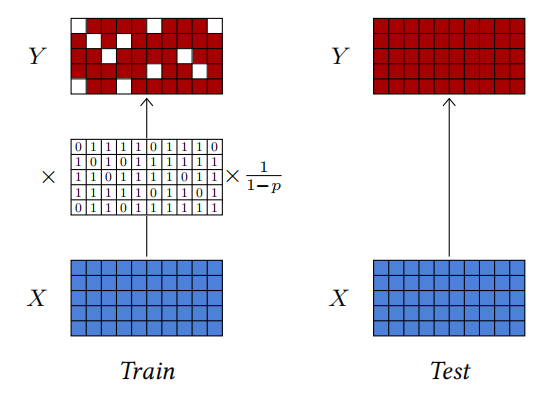
\includegraphics[width=0.9\textwidth]{fig/fig4.7.png}
    \caption[Dropout]{Dropout 可以处理任意形状的张量。在训练期间(左),它以概率 $p$ 将激活随机设置为零,并应用乘法因子来保持预期值不变。在测试期间(右),它保持所有激活不变。}
    \label{fig4.7}
\end{figure}

使用 Dropout 的动机在于促进有意义的单个激活,并阻止群体表征。由于一组 $k$ 个激活通过 Dropout 层保持完整的概率为 $(1-p)^k$,因此联合表征变得不可靠,从而使训练过程避免使用它们。Dropout 也可以被视为一种噪声注入,使训练更加稳健。

在处理图像和二维张量时,信号的短期相关性和由此产生的冗余抵消了 Dropout 的影响,因为可以从其邻居中推断出设置为零的激活。 因此,二维张量的 Dropout 将整个通道设置为零,而不是单个激活(见图 \ref{fig4.8})。

\begin{figure}
    \centering
    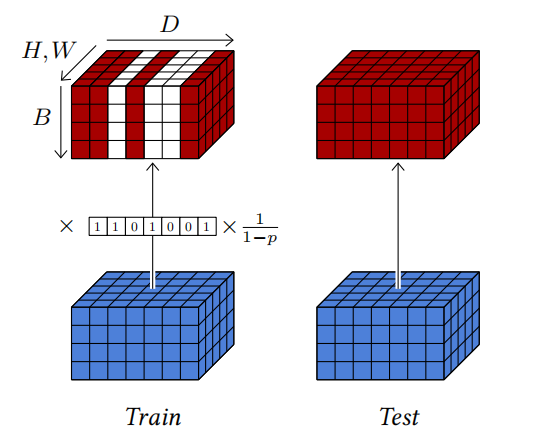
\includegraphics[width=0.9\textwidth]{fig/fig4.8.png}
    \caption[二维 Dropout]{诸如图像之类的二维信号通常表现出很强的短期相关性,并且可以从其邻居中推断出各个激活。这种冗余消除了标准非结构化 Dropout 的影响,因此二维张量的常用 Dropout 层会丢弃整个通道而不是单个值。}
    \label{fig4.8}
\end{figure}

尽管 Dropout 通常用于改进训练而在推理过程中处于非活动状态,但它可以在某些设置中用作随机化策略,例如,根据经验估计置信度分数 \citep{arxiv-1506.02142}。

\section{归一化层}\label{sec4.6}

在深度架构训练中,一类重要的操作是\keyterm{归一化层},它强制对一组激活函数的经验平均值和方差进行标准化。

这一类别的主要层是\keyterm{批量归一化} \citep{43442},它是唯一一个处理整批数据而不是单个样本的标准层。它由元参数 $D$ 和两组可训练标量参数 $\beta_1,\dots,\beta_D$ 和 $\gamma_1,\dots,\gamma_D$ 参数化。

给定一个由 $B$ 个 $D$ 维样本 $x_1,\dots,x_B$ 组成的批数据,它首先计算每个 D 分量的经验平均值 $\hat{m}_d$ 和方差 $\hat{v}_d$:
\begin{align*}
    \hat{m}_d &= \frac{1}{B}\sum_{b=1}^{B}x_{b,d} \\
    \hat{v}_d &= \frac{1}{B}\sum_{b=1}^{B}(x_{b,d}-\hat{m}_d)^2
\end{align*}
从中计算每个分量 $x_{b,d}$ 的归一化值 $z_{b,d}$,经验平均值为 $0$,方差为 $1$,并由此得出最终结果值 $y_{b,d}$,平均值为 $\beta_d$,标准差为 $\gamma_d$:
\begin{align*}
    \forall b, \quad z_{b,d} &= \frac{x_{b,d}-\hat{m}_d}{\sqrt{\hat{v}_d+\epsilon}}\\
    y_{b,d} &= \gamma_dz_{b,d}+\beta_d
\end{align*}
由于此标准化是跨批次定义的,因此仅在训练期间完成。在测试过程中,该层根据整个训练集上偏移平均值估计的 $m_d$ 和 $v_d$ 来转换各个样本,这可以归结为每个组件的固定仿射变换。

批量归一化背后的动机是避免网络早期层在训练期间的缩放变化影响到后续所有层,这些层随后需要相应地调整它们的可训练参数。尽管实际的作用机制可能比这一初衷更加复杂,但这种层显著地简化了深度模型的训练过程。

在二维张量的情况下,为了遵循卷积层处理所有位置的相似性原则,归一化是按通道进行的,覆盖所有二维位置,而 $\beta$ 和 $\gamma$ 仍然是 $D$ 维向量,因此缩放/偏移不依赖于二维位置。因此,如果待处理张量的形状为 $B \times D \times H \times W$,对于 $d = 1,\dots,D$,该层根据相应的 $B \times H \times W$ 切片计算 $(\hat{m}_d,\hat{v}_d)$,对其进行归一化。最后使用可训练参数 $\beta_d$ 和 $\gamma_d$ 缩放和偏移其分量。

\begin{figure}
    \centering
    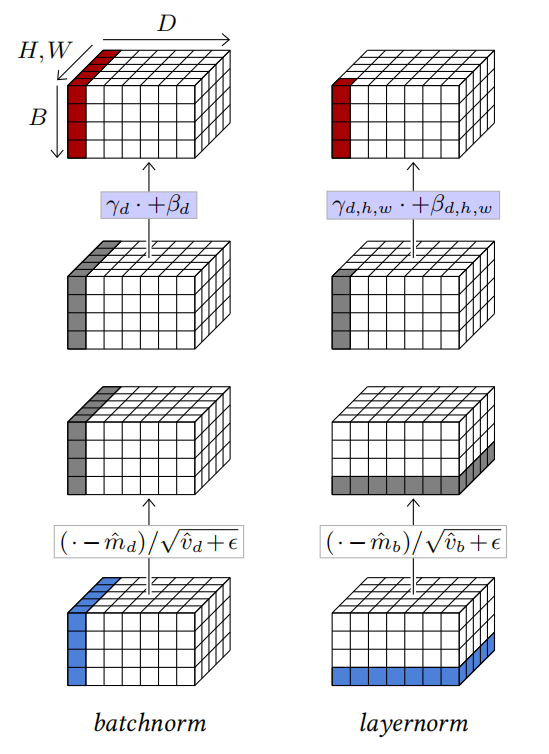
\includegraphics[width=0.9\textwidth]{fig/fig4.9.png}
    \caption[批量归一化]{批量归一化(左)对给定 $d$ 的每组激活的均值和方差进行归一化,并使用每个 $d$ 的学习参数缩放/偏移同一组激活。层归一化(右)对特定 $b$ 的每组激活进行归一化,并使用由相同索引的学习参数对给定 $d,h,w$ 的每组激活进行缩放/偏移。}
    \label{fig4.9}
\end{figure}

因此,给定一个 $B \times D$ 张量,批量归一化会在 $b$ 上对其进行归一化,并根据 $d$ 对其进行缩放/偏移,这可以通过 $\gamma$ 的逐元素乘积和与 $\beta$ 的求和来实现。给定 $B \times D \times H \times W$ 张量,它会根据 $b,h,w$ 进行归一化,并根据 $d$ 进行缩放/偏移(参见图 \ref{fig4.9},左图)。

这种方法可以根据这些维度进行泛化。例如,\keyterm{层归一化} \citep{arxiv-1607.06450} 计算单个样本所有分量的矩,并进行归一化,然后对各个分量分别进行缩放和偏移(参见图 \ref{fig4.9},右图)。因此,给定一个 $B \times D$ 的张量,它会根据 $d$ 进行归一化,并且根据相同的维度进行缩放/偏移。给定一个 $B \times D \times H \times W$ 的张量,它会根据 $d,h,w$ 进行归一化,并且根据同样的维度进行缩放/偏移。

\newpage

与批量归一化不同的是,由于层归一化单独处理每个样本,因此它在训练和测试期间的表现是相同的。

\section{跳跃连接}\label{sec4.7}

\section{注意力层}\label{sec4.8}

\section{Token 嵌入}\label{sec4.9}

\section{位置编码}\label{sec4.10}
% !TeX root = ../main.tex
\chapter{架构}\label{ch5}

多年来,深度学习领域已经为每个应用领域开发了多种深度架构,这些架构在多个人们关注的标准方面表现出良好的折中:例如 训练便捷性、预测准确性、内存占用、计算成本、可扩展性等。

\section{多层感知机}\label{sec5.1}

最简单的深度架构是\keyterm{多层感知机}(\keyterm{MLP}),它由一系列\keyterm{全连接层}组成,层与层之间通过\keyterm{激活函数}分隔。请参见图 \ref{fig5.1} 中的示例。由于历史原因,在这样的模型中,\keyterm{隐藏层}的数量指的是线性层的数量,不包括最后一层。

\begin{figure}
    \centering
    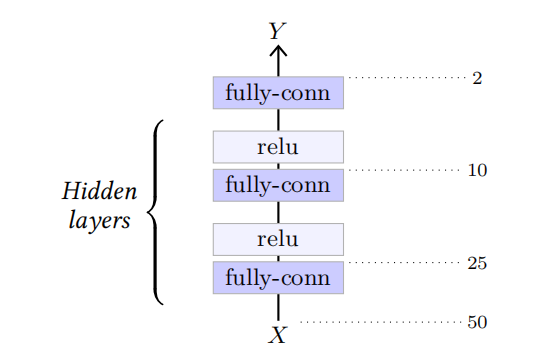
\includegraphics[width=0.9\textwidth]{fig/fig5.1.png}
    \caption[多层感知机]{该多层感知器以大小为 $50$ 的一维张量作为输入,由三个全连接层组成,输出维度分别为 $25$、$10$ 和 $2$,前两个层后面是 ReLU 层。}
    \label{fig5.1}
\end{figure}

一个关键的理论成果是\keyterm{通用逼近定理} \citep{Cybenko1989},该定理指出,如果激活函数 $\sigma$ 是连续的且非多项式的,那么任意连续函数 $f$ 都可以在紧致域上被形式为 $l_2 \circ \sigma \circ l_1$ 的模型任意精确地一致逼近,其中紧致域是有界的并包含其边界,$l_1$ 和 $l_2$ 是仿射的。这样的模型是一个只有单个隐藏层的多层感知机(\keyterm{MLP}),这个结果意味着它可以近似任何具有实用价值的东西。然而,这种逼近成立的条件是第一个线性层的输出维度可以任意大。

尽管 MLP 很简单,但当要处理的信号维度不太大时,它仍然是一个重要的工具。

\section{卷积网络}\label{sec5.2}

\section{注意力模型}\label{sec5.3}

%%%%%%%%%%%%%%%%%%%%%%%%%%%%%%%%%%%%%%%%%%%%%%%%%%%%%%%%%%%%%%%%%%%%%%%%%%%%%%%%%%%%%%%%%%%

\part{应用}

% !TeX root = ../main.tex
\chapter{预测}\label{ch6}

第一类应用,例如面部识别、情感分析、对象检测或语音识别,需要从可用信号中预测未知值。

\section{图像去噪}\label{sec6.1}

将深度模型直接应用于图像处理的一个具体应用是利用图像的统计结构中的冗余来从退化中恢复图像。例如,在一张灰度图片中,向日葵的花瓣可以以高置信度进行着色,而几何形状的纹理,例如低光、颗粒状图片上的桌子,可以通过在可能均匀的大区域上进行平均来校正。

\keyterm{去噪自动编码器}是一种模型,它将受损的信号 $\tilde{X}$ 作为输入,并计算出原始信号 $X$ 的估计。对于图像,它是一个可以集成跳跃连接的卷积网络,特别是组合早期获得的相同分辨率的表示 在模型的后期,以及注意层,以方便考虑彼此相距较远的元素。对于图像来说,它是一个卷积网络,可能会集成跳跃连接,尤其是为了组合在模型前期和后期获得的同一分辨率的表示,以及注意力层,以便考虑彼此距离较远的元素。

这样的模型是通过收集大量干净样本及其对应的受损输入来训练的。后者可以在低光或聚焦不足等退化条件下捕获,也可以通过算法生成,例如通过将干净的样本转换为灰度、减小其大小或使用有损压缩方法对其进行激进压缩。

去噪自动编码器的标准训练过程使用所有像素的 MSE 损失之和,在这种情况下,在这种情况下,模型的目标是在给定受损图片的情况下计算出最佳的平均干净图片,即 $E[X \mid \tilde{X}]$。当 $X$ 不完全由 $\tilde{X}$ 确定时,这个量可能是有问题的,在这种情况下,生成信号的某些部分可能是不切实际的、模糊的平均值。

\section{图像分类}\label{sec6.2}

图像\keyterm{分类}是从图像中提取语义的最简单策略,包括在给定输入图像的情况下,从有限的、预定义数量的类别中预测类别。

此任务的标准模型是卷积网络,例如 ResNets(详见 \ref{sec5.2} 节),以及基于注意力的模型,例如 ViT(详见 \ref{sec5.3} 节)。这些模型生成一个 logits 向量,其维度与类别的数量一样多。

训练过程只是最小化交叉熵损失(详见 \ref{sec3.1} 节)。通常,可以通过\keyterm{数据增强}来提高性能,数据增强包括使用手工设计的随机变换修改训练样本,这些变换不会改变图像的语义内容,例如裁剪、缩放、镜像或颜色变化。

\section{对象检测}\label{sec6.3}

图像理解的一个更复杂的任务是\keyterm{对象检测},其目标是在给定输入图像的情况下预测感兴趣对象的类别和位置。

对象位置被形式化为矩形边界框的四个坐标 $(x_1,y_1,x_2,y_2)$,与每个训练图像相关联的真实值是这样的边界框列表,每个边界框都标有其中包含的对象的类别。

解决这一任务的标准方法,例如通过\keyterm{单次检测器}(\keyterm{SSD})\citep{arxiv-1512.02325},是使用卷积神经网络产生一系列大小为 $D_s \times H_s \times W_s$ 的图像表示 $Z_s$,其中 $s = 1, \dots, S$。空间分辨率 $H_s \times W_s$ 逐渐减小,直至 $s = S$ 时缩小为 $1 \times 1$(见图 \ref{fig6.1})。这些张量中的每一个都完全覆盖输入图像,因此 $h,w$ 索引对应于将图像划分为规则正方形,当 $s$ 增加时,规则正方形会变得更加粗糙。

\begin{figure}
    \centering
    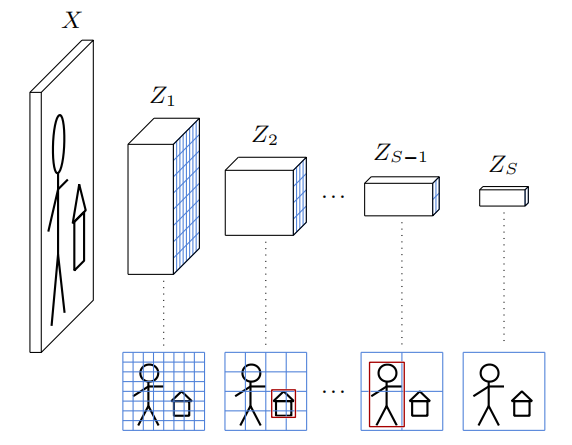
\includegraphics[width=0.9\textwidth]{fig/fig6.1.png}
    \caption[卷积物体检测器]{卷积对象检测器处理输入图像以生成一系列分辨率递减的表示。它在每个尺度 $s$ 上为每个 $h,w$ 计算预定义数量的边界框,这些边界框的中心位于与该单元相对应的图像区域中,并且其大小适合其接受范围。每个预测均采用估计值 ($\hat{x}_1, \hat{x}_2, \hat{y}_1, \hat{y}_2$) 的形式,由上面的红色框表示,以及 $C + 1$ 个 Logits 组成的向量,表示 $C$ 个感兴趣的类别和一个附加的``无对象''类别。}
    \label{fig6.1}
\end{figure}

如 \ref{sec4.2} 节和图 \ref{fig4.4} 所示,由于\keyterm{卷积层}的连续性,特征向量 $(Z_s[0,h,w],\dots,Z_s[D_s-1,h,w])$ 是图像区域的描述符,称为其\keyterm{感受野},它比这个正方形大,但以它为中心。这导致任何边界框 $(x_1,x_2,y_1,y_2)$ 与 $s,h,w$ 的明确匹配,分别由 $\text{max}(x_2-x_1,y_2-y_1), \frac{y_1+y_2}{2}, \frac{x_1+x_2}{2}$ 确定。

检测是通过添加 $S$ 个卷积层来实现的,每个卷积层处理一个 $Z_s$ 并为每个张量索引 $h,w$ 计算边界框的坐标和相关的 logits 值。如果有 $C$ 个对象类别,就会有 $C + 1$ 个 logits 值,额外的一个表示``无对象''。因此,每个附加卷积层都有 $4 + C + 1$ 个输出通道。SSD 算法特别为每个 $s,h,w$ 生成多个边界框,每个边界框专用于硬编码的长宽比范围。

由于使用边界框进行标注需要人工缓慢地干预,因此创建用于对象检测的训练集成本较高。为了缓解这个问题,标准方法是从一个在大型分类数据集上\keyterm{预训练}过的卷积模型开始,比如原始 SSD 使用 VGG-16,然后用额外的卷积层替换其最后的全连接层。令人惊讶的是,尽管对象检测任务涉及到几何量的回归,但仅为分类任务训练的模型所学习到的特征表示却可以重用于对象检测。

在训练过程中,每个真实边界框都与其 $s,h,w$ 相关联,并引入一个损失项,该损失项由 logits 的交叉熵损失和边界框坐标的回归损失(例如 MSE)组成。其他没有边界框匹配的 $s,h,w$ 会引发仅交叉熵惩罚来预测``无对象''类。

\begin{figure}
    \centering
    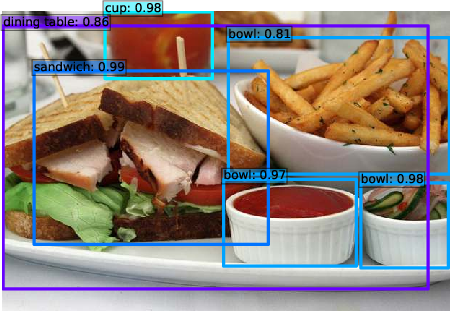
\includegraphics[width=0.8\textwidth]{fig/fig6.2-1.png}
    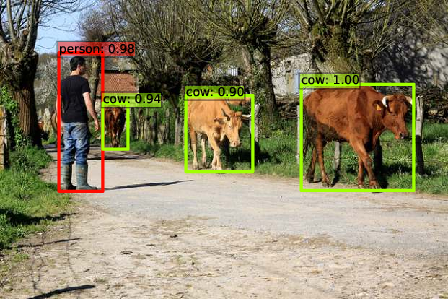
\includegraphics[width=0.8\textwidth]{fig/fig6.2-2.png}
    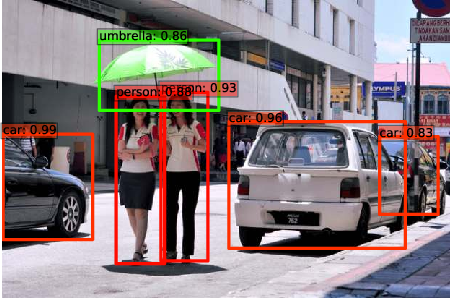
\includegraphics[width=0.8\textwidth]{fig/fig6.2-3.png}
    \caption[使用 SSD 进行物体检测]{使用单次检测器进行物体检测的示例 \citep{arxiv-1512.02325}}
    \label{fig6.2}
\end{figure}

\section{语义分割}\label{sec6.4}

图像理解中最精细的预测任务是\keyterm{语义分割},它涉及预测每个像素所属物体的类别。这可以通过一个标准的卷积神经网络来实现,该网络输出一个卷积图,其中包含与类别数量相同的通道,为每个像素携带估计的 logits 值。

例如,一个标准的残差网络可以生成与其输入相同分辨率的密集输出,就像物体检测一样,这项任务需要在多个尺度上进行操作。这是必要的,以便任何对象或信息丰富的子部分,无论其大小如何,都可以通过单个张量位置的特征表示在模型中的某个位置捕获。因此,这项任务的标准架构会通过一系列\keyterm{卷积层}来缩小图像尺寸,以增大激活的感受野,然后通过一系列\keyterm{转置卷积层}或其他上采样方法(如双线性插值)来重新放大图像,以便进行高分辨率的预测。

\begin{figure}
    \centering
    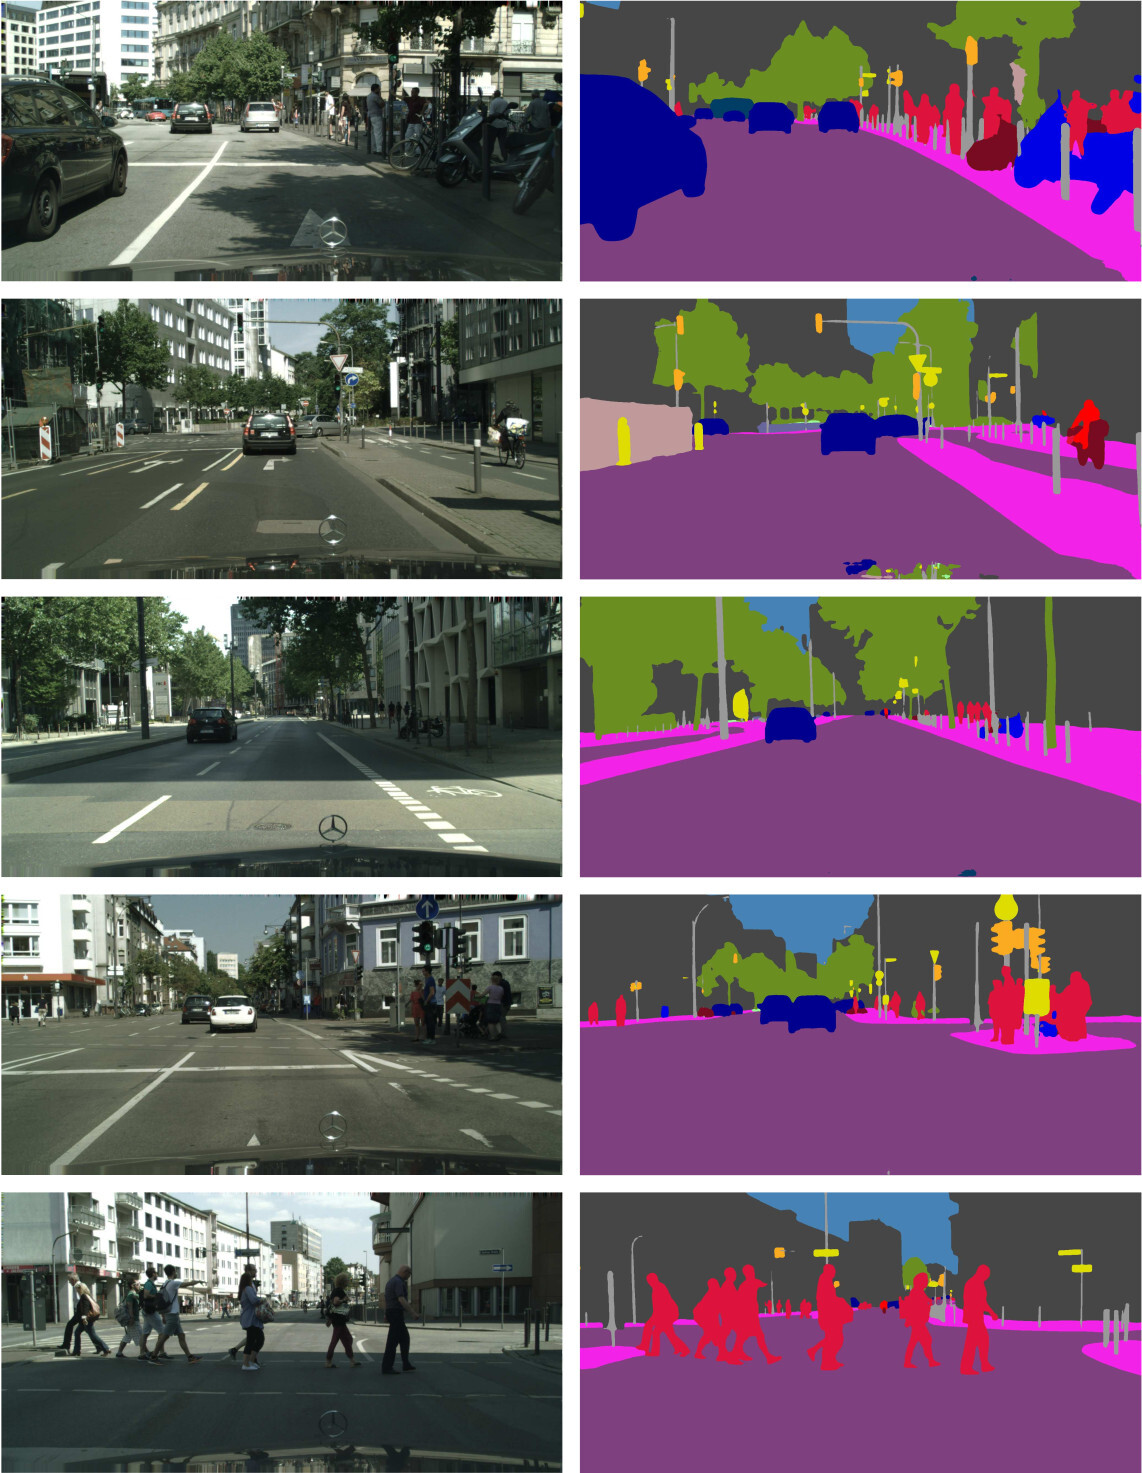
\includegraphics[width=0.9\textwidth]{fig/fig6.3.png}
    \caption[用 PSP 进行语义分割]{金字塔场景分析网络的语义分割结果 \citep{arxiv-1612.01105}}
    \label{fig6.3}
\end{figure}

然而,严格的下采样-上采样架构不允许在进行最终预测时进行细粒度的操作,因为所有的信号在某个时刻都通过了低分辨率的表示。应用这种下采样-上采样的模型通过从缩小之前的特定分辨率的层到放大之后的相同分辨率的层的\keyterm{跳跃连接}来连续缓解这些问题 \citep{arxiv-1411.4038, arxiv-1505.04597}。并行执行此操作的模型,在卷积主干之后,在进行最终的每像素预测之前,在上采样后连接所得的多尺度表示 \citep{arxiv-1612.01105}。

训练是通过对所有像素求和的标准交叉熵来实现的。与对象检测一样,为了弥补分割真值数据有限的问题,训练可以从在大规模图像分类数据集上\keyterm{预训练的网络}开始。

\section{语音识别}\label{sec6.5}

\keyterm{语音识别}包括将声音样本转换为单词序列。历史上有很多解决这个问题的方法,但 Radford \cite{arxiv-2212.04356} 最近提出的一种概念上简单的方法包括将其视为序列到序列的翻译,然后使用标准的基于注意力的 \keyterm{Transformer} 来解决它,如 \ref{sec5.3} 节中所述。

他们的模型首先将声音信号转换为频谱图,该频谱图是一个一维序列 $T \times D$,在每个时间步编码 $D$ 个频带中的能量向量。 关联的文本使用 \keyterm{BPE 分词器}进行编码(参见 \ref{sec3.2} 节)。

频谱图通过几个一维\keyterm{卷积层}进行处理,并将得到的表示输入到 Transformer 的编码器中。解码器直接生成离散的标记序列,其对应于训练期间考虑的可能任务之一。考虑多个目标:英语或非英语文本的转录、从任何语言到英语的翻译、或非语音序列的检测,例如背景音乐或环境噪音。

这种方法可以利用极其庞大的数据集,将多种类型的声源与不同的基本事实相结合。

值得注意的是,尽管这种方法的最终目标是在给定输入信号的情况下产生尽可能确定的翻译,但它形式上是对声音样本条件下的文本分布进行采样,因此这是一个合成过程。事实上,解码器与 \ref{sec7.1} 节的生成模型极其相似。

\section{文本图像表示}\label{sec6.6}

一种强大的图像理解方法包括学习一致的图像和文本表示,这样一来,无论是一幅图像还是其文本描述,都会被映射到同一个特征向量上。

\cite{arxiv-2103.00020} 提出的\keyterm{对比语言-图像预训练}(\keyterm{CLIP})结合了图像编码器 $f$,即 ViT 和文本编码器 $g$,即 GPT。两者均可参见 \ref{sec5.3} 节。

为了将 GPT 重新用作文本编码器,而不是标准的自回归模型,他们向输入序列添加了``句末''标记,并使用最后一层中该标记的表示作为嵌入。 其尺寸在 $512$ 到 $1024$ 之间,具体取决于配置。

这两个模型使用从 Internet 收集的 4 亿张图像文本对 $(i_k,t_k)$ 从头开始训练。训练过程遵循标准的小批量随机梯度下降法,但依赖于\keyterm{对比损失}。对于小批量中的 $N$ 对图像和文本,都会计算出相应的嵌入向量,并计算每对图像与文本嵌入向量之间的余弦相似度,还会计算跨对之间的相似度,从而得到一个 $N \times N$ 矩阵的相似度得分:
\[l_{m,n} = f(i_m) \cdot g(t_n), m = 1,\dots,N, n = 1,\dots,N\]
模型使用交叉熵进行训练,$\forall n$ 值 $l_{1,n},\dots,l_{N,n}$ 被解释为预测 $n$ 的 logit 分数,$l_{n,1},\dots,l_{n,N}$ 与之类似。这意味着 $\forall n,m, \text{s.t.} n \ne m$ 时,相似度 $l_{n,n}$ 严格大于 $l_{n,m}$ 和 $l_{m,n}$。

训练完成后,该模型可用于\keyterm{零样本预测},即在没有训练样例的情况下对信号进行分类。方法是定义一系列带有文本描述的候选类别,并计算图像嵌入向量与这些描述中每一个嵌入向量的相似度(见图 \ref{fig6.4})。

\begin{figure}
    \centering
    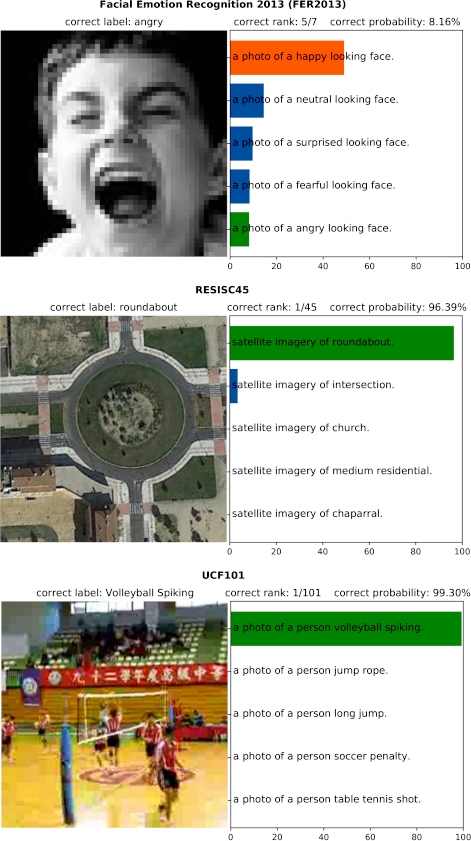
\includegraphics[width=0.9\textwidth]{fig/fig6.4.png}
    \caption[CLIP 零样本预测]{CLIP 文本图像嵌入 \citep{arxiv-2103.00020} 允许通过预测哪类描述嵌入与图像嵌入最一致来进行零样本预测。}
    \label{fig6.4}
\end{figure}

此外,由于文本描述通常更为详细,这样的模型需要捕捉图像更丰富的表示,并且识别出超出常规分类所需的线索。这意味着在一些具有挑战性的数据集上,例如专门设计用来降低或消除标准预测器依赖的线索的数据集 ImageNet Adversarial \citep{arxiv-1907.07174},该模型展现出了出色的性能。

\section{强化学习}\label{sec6.7}

\begin{figure}
    \centering
    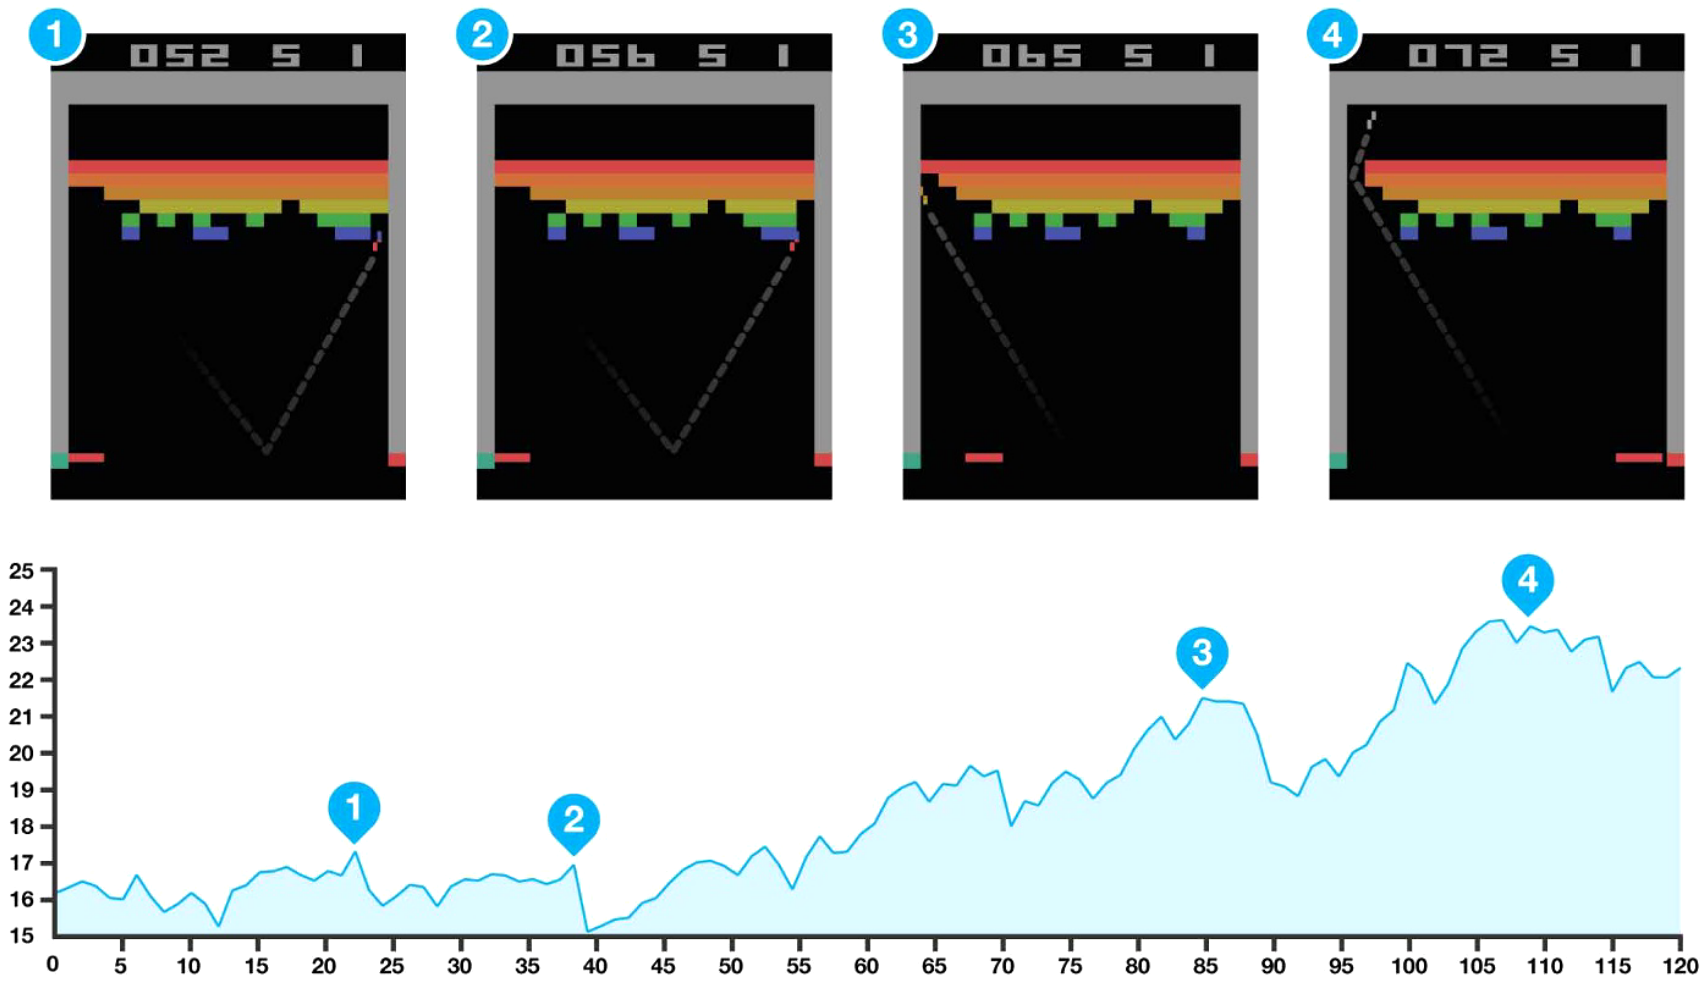
\includegraphics[width=0.9\textwidth]{fig/fig6.5.png}
    \caption[DQN 状态值演化]{该图显示了打砖块游戏期间状态值 $V(S_t)=\max_aQ(S_t,a)$ 的演变。时间点 (1) 和 (2) 处的尖峰对应于清除砖块,在时间点 (3) 处,砖块即将突破顶线,在 (4) 处确实突破了顶线,这确保了未来的高奖励 \citep{nature14236}。}
    \label{fig6.5}
\end{figure}
% !TeX root = ../main.tex
\chapter{合成}

%%%%%%%%%%%%%%%%%%%%%%%%%%%%%%%%%%%%%%%%%%%%%%%%%%%%%%%%%%%%%%%%%%%%%%%%%%%%%%%%%%%%%%%%%%%

\bibliography{main}


\printindex

%%%%%%%%%%%%%%%%%%%%%%%%%%%%%%%%%%%%%%%%%%%%%%%%%%%%%%%%%%%%%%%%%%%%%%%%%%%%%%%%%%%%%%%%%%%

\newpage

\vspace*{\stretch{1}}

\ifdefined\draft
\begin{center}
  {\color{red} (draft, do not circulate)}
\end{center}
\else
本书根据
\href{https://creativecommons.org/licenses/by-nc-sa/4.0/}{Creative
  Commons BY-NC-SA 4.0 国际许可}授权
\fi

\begin{center}
    翻译自 \href{https://fleuret.org/public/lbdl.pdf}{V1.1.1} - 2023.09.20
\end{center}

\vspace*{\stretch{1}}

%%%%%%%%%%%%%%%%%%%%%%%%%%%%%%%%%%%%%%%%%%%%%%%%%%%%%%%%%%%%%%%%%%%%%%%%%%%%%%%%%%%%%%%%%%%

\checknbdrafts

\end{document}
